% Options for packages loaded elsewhere
\PassOptionsToPackage{unicode}{hyperref}
\PassOptionsToPackage{hyphens}{url}
%
\documentclass[
]{article}
\usepackage{amsmath,amssymb}
\usepackage{lmodern}
\usepackage{iftex}
\ifPDFTeX
  \usepackage[T1]{fontenc}
  \usepackage[utf8]{inputenc}
  \usepackage{textcomp} % provide euro and other symbols
\else % if luatex or xetex
  \usepackage{unicode-math}
  \defaultfontfeatures{Scale=MatchLowercase}
  \defaultfontfeatures[\rmfamily]{Ligatures=TeX,Scale=1}
\fi
% Use upquote if available, for straight quotes in verbatim environments
\IfFileExists{upquote.sty}{\usepackage{upquote}}{}
\IfFileExists{microtype.sty}{% use microtype if available
  \usepackage[]{microtype}
  \UseMicrotypeSet[protrusion]{basicmath} % disable protrusion for tt fonts
}{}
\makeatletter
\@ifundefined{KOMAClassName}{% if non-KOMA class
  \IfFileExists{parskip.sty}{%
    \usepackage{parskip}
  }{% else
    \setlength{\parindent}{0pt}
    \setlength{\parskip}{6pt plus 2pt minus 1pt}}
}{% if KOMA class
  \KOMAoptions{parskip=half}}
\makeatother
\usepackage{xcolor}
\usepackage[margin=1in]{geometry}
\usepackage{color}
\usepackage{fancyvrb}
\newcommand{\VerbBar}{|}
\newcommand{\VERB}{\Verb[commandchars=\\\{\}]}
\DefineVerbatimEnvironment{Highlighting}{Verbatim}{commandchars=\\\{\}}
% Add ',fontsize=\small' for more characters per line
\usepackage{framed}
\definecolor{shadecolor}{RGB}{248,248,248}
\newenvironment{Shaded}{\begin{snugshade}}{\end{snugshade}}
\newcommand{\AlertTok}[1]{\textcolor[rgb]{0.94,0.16,0.16}{#1}}
\newcommand{\AnnotationTok}[1]{\textcolor[rgb]{0.56,0.35,0.01}{\textbf{\textit{#1}}}}
\newcommand{\AttributeTok}[1]{\textcolor[rgb]{0.77,0.63,0.00}{#1}}
\newcommand{\BaseNTok}[1]{\textcolor[rgb]{0.00,0.00,0.81}{#1}}
\newcommand{\BuiltInTok}[1]{#1}
\newcommand{\CharTok}[1]{\textcolor[rgb]{0.31,0.60,0.02}{#1}}
\newcommand{\CommentTok}[1]{\textcolor[rgb]{0.56,0.35,0.01}{\textit{#1}}}
\newcommand{\CommentVarTok}[1]{\textcolor[rgb]{0.56,0.35,0.01}{\textbf{\textit{#1}}}}
\newcommand{\ConstantTok}[1]{\textcolor[rgb]{0.00,0.00,0.00}{#1}}
\newcommand{\ControlFlowTok}[1]{\textcolor[rgb]{0.13,0.29,0.53}{\textbf{#1}}}
\newcommand{\DataTypeTok}[1]{\textcolor[rgb]{0.13,0.29,0.53}{#1}}
\newcommand{\DecValTok}[1]{\textcolor[rgb]{0.00,0.00,0.81}{#1}}
\newcommand{\DocumentationTok}[1]{\textcolor[rgb]{0.56,0.35,0.01}{\textbf{\textit{#1}}}}
\newcommand{\ErrorTok}[1]{\textcolor[rgb]{0.64,0.00,0.00}{\textbf{#1}}}
\newcommand{\ExtensionTok}[1]{#1}
\newcommand{\FloatTok}[1]{\textcolor[rgb]{0.00,0.00,0.81}{#1}}
\newcommand{\FunctionTok}[1]{\textcolor[rgb]{0.00,0.00,0.00}{#1}}
\newcommand{\ImportTok}[1]{#1}
\newcommand{\InformationTok}[1]{\textcolor[rgb]{0.56,0.35,0.01}{\textbf{\textit{#1}}}}
\newcommand{\KeywordTok}[1]{\textcolor[rgb]{0.13,0.29,0.53}{\textbf{#1}}}
\newcommand{\NormalTok}[1]{#1}
\newcommand{\OperatorTok}[1]{\textcolor[rgb]{0.81,0.36,0.00}{\textbf{#1}}}
\newcommand{\OtherTok}[1]{\textcolor[rgb]{0.56,0.35,0.01}{#1}}
\newcommand{\PreprocessorTok}[1]{\textcolor[rgb]{0.56,0.35,0.01}{\textit{#1}}}
\newcommand{\RegionMarkerTok}[1]{#1}
\newcommand{\SpecialCharTok}[1]{\textcolor[rgb]{0.00,0.00,0.00}{#1}}
\newcommand{\SpecialStringTok}[1]{\textcolor[rgb]{0.31,0.60,0.02}{#1}}
\newcommand{\StringTok}[1]{\textcolor[rgb]{0.31,0.60,0.02}{#1}}
\newcommand{\VariableTok}[1]{\textcolor[rgb]{0.00,0.00,0.00}{#1}}
\newcommand{\VerbatimStringTok}[1]{\textcolor[rgb]{0.31,0.60,0.02}{#1}}
\newcommand{\WarningTok}[1]{\textcolor[rgb]{0.56,0.35,0.01}{\textbf{\textit{#1}}}}
\usepackage{longtable,booktabs,array}
\usepackage{calc} % for calculating minipage widths
% Correct order of tables after \paragraph or \subparagraph
\usepackage{etoolbox}
\makeatletter
\patchcmd\longtable{\par}{\if@noskipsec\mbox{}\fi\par}{}{}
\makeatother
% Allow footnotes in longtable head/foot
\IfFileExists{footnotehyper.sty}{\usepackage{footnotehyper}}{\usepackage{footnote}}
\makesavenoteenv{longtable}
\usepackage{graphicx}
\makeatletter
\def\maxwidth{\ifdim\Gin@nat@width>\linewidth\linewidth\else\Gin@nat@width\fi}
\def\maxheight{\ifdim\Gin@nat@height>\textheight\textheight\else\Gin@nat@height\fi}
\makeatother
% Scale images if necessary, so that they will not overflow the page
% margins by default, and it is still possible to overwrite the defaults
% using explicit options in \includegraphics[width, height, ...]{}
\setkeys{Gin}{width=\maxwidth,height=\maxheight,keepaspectratio}
% Set default figure placement to htbp
\makeatletter
\def\fps@figure{htbp}
\makeatother
\setlength{\emergencystretch}{3em} % prevent overfull lines
\providecommand{\tightlist}{%
  \setlength{\itemsep}{0pt}\setlength{\parskip}{0pt}}
\setcounter{secnumdepth}{-\maxdimen} % remove section numbering
\ifLuaTeX
  \usepackage{selnolig}  % disable illegal ligatures
\fi
\IfFileExists{bookmark.sty}{\usepackage{bookmark}}{\usepackage{hyperref}}
\IfFileExists{xurl.sty}{\usepackage{xurl}}{} % add URL line breaks if available
\urlstyle{same} % disable monospaced font for URLs
\hypersetup{
  pdftitle={Dissertation},
  pdfauthor={Imogen Whitehead},
  hidelinks,
  pdfcreator={LaTeX via pandoc}}

\title{Dissertation}
\author{Imogen Whitehead}
\date{}

\begin{document}
\maketitle

{
\setcounter{tocdepth}{2}
\tableofcontents
}
\begin{Shaded}
\begin{Highlighting}[]
\CommentTok{\#number\_sections: yes}
    \CommentTok{\#code\_folding: hide}
    \CommentTok{\#theme: cerulean}
\CommentTok{\#html\_document:}

\CommentTok{\#message=FALSE means some output messages aren\textquotesingle{}t printed in the knitted HTML document}

\NormalTok{knitr}\SpecialCharTok{::}\NormalTok{opts\_chunk}\SpecialCharTok{$}\FunctionTok{set}\NormalTok{(}\AttributeTok{echo =} \ConstantTok{FALSE}\NormalTok{, }\AttributeTok{warning=}\ConstantTok{FALSE}\NormalTok{) }
\CommentTok{\#include=FALSE, echo=FALSE and warning=FALSE ensure the code and any error messages aren\textquotesingle{}t shown in the output HTML file}

\CommentTok{\#message=FALSE means no output messages are printed on the knitted HMTL file}
\CommentTok{\#loading any necessary packages}
\FunctionTok{library}\NormalTok{(dplyr)}
\FunctionTok{library}\NormalTok{(tidyverse) }
\FunctionTok{library}\NormalTok{(knitr)}
\FunctionTok{library}\NormalTok{(readr)}
\FunctionTok{library}\NormalTok{(ggplot2)}
\FunctionTok{library}\NormalTok{(bbmle)}
\FunctionTok{library}\NormalTok{(mizer) }
\FunctionTok{library}\NormalTok{(Hmisc)}
\FunctionTok{library}\NormalTok{(lme4)}
\FunctionTok{library}\NormalTok{(RColorBrewer)}
\FunctionTok{library}\NormalTok{(viridis)}
\FunctionTok{library}\NormalTok{(hexbin)}
\end{Highlighting}
\end{Shaded}

\begin{Shaded}
\begin{Highlighting}[]
\FunctionTok{load}\NormalTok{(}\StringTok{"stomach\_dataset.Rdata"}\NormalTok{)}
\CommentTok{\#loading the dataset to be used in analysis (the dataset is already named stom\_df)}

\NormalTok{df }\OtherTok{\textless{}{-}}\NormalTok{ stom\_df }\SpecialCharTok{\%\textgreater{}\%} \FunctionTok{transmute}\NormalTok{(haul\_id, ices\_rectangle, year, pred\_species, }
\NormalTok{                            pred\_weight\_g, pred\_length\_cm, prey\_weight\_g, }
                            \AttributeTok{prey\_type =}\NormalTok{ prey\_funcgrp, }\AttributeTok{indiv\_prey\_weight =}\NormalTok{ prey\_ind\_weight\_g, }
\NormalTok{                            prey\_count, n\_stomachs, }\AttributeTok{no.\_prey\_per\_stmch =}\NormalTok{ prey\_count}\SpecialCharTok{/}\NormalTok{n\_stomachs, ppmr) }
\CommentTok{\#creating a new data set called \textquotesingle{}df\textquotesingle{} which only contains certain selected columns}

\NormalTok{df }\OtherTok{\textless{}{-}}\NormalTok{ df[df}\SpecialCharTok{$}\NormalTok{indiv\_prey\_weight }\SpecialCharTok{!=} \DecValTok{0}\NormalTok{, ]}
\NormalTok{df }\OtherTok{\textless{}{-}}\NormalTok{ df[df}\SpecialCharTok{$}\NormalTok{pred\_weight\_g }\SpecialCharTok{!=} \DecValTok{0}\NormalTok{, ]}
\NormalTok{df }\OtherTok{\textless{}{-}}\NormalTok{ df[df}\SpecialCharTok{$}\NormalTok{indiv\_prey\_weight }\SpecialCharTok{!=} \ConstantTok{Inf}\NormalTok{, ]}
\CommentTok{\#Removes any points where the prey weight = Inf or 0, or the predator weight = 0}
\end{Highlighting}
\end{Shaded}

\begin{Shaded}
\begin{Highlighting}[]
\NormalTok{renamed\_df }\OtherTok{=}\NormalTok{ df }\SpecialCharTok{\%\textgreater{}\%} 
  \FunctionTok{mutate}\NormalTok{(}\AttributeTok{pred\_species =} \FunctionTok{replace}\NormalTok{(pred\_species, }
\NormalTok{                                pred\_species }\SpecialCharTok{==} \StringTok{"Micromesistius poutassou"}\NormalTok{, }\StringTok{"Blue Whiting"}\NormalTok{)) }\SpecialCharTok{\%\textgreater{}\%}
\CommentTok{\#  mutate(pred\_species = replace(pred\_species, pred\_species == "Capros apers", "Boarfish")) \%\textgreater{}\%}
  \FunctionTok{mutate}\NormalTok{(}\AttributeTok{pred\_species =} \FunctionTok{replace}\NormalTok{(pred\_species, pred\_species }\SpecialCharTok{==} \StringTok{"Gadus morhua"}\NormalTok{, }\StringTok{"Cod"}\NormalTok{)) }\SpecialCharTok{\%\textgreater{}\%} 
  \FunctionTok{mutate}\NormalTok{(}\AttributeTok{pred\_species =} \FunctionTok{replace}\NormalTok{(pred\_species, pred\_species }\SpecialCharTok{==} \StringTok{"Limanda limanda"}\NormalTok{, }\StringTok{"Common Dab"}\NormalTok{)) }\SpecialCharTok{\%\textgreater{}\%}
  \FunctionTok{mutate}\NormalTok{(}\AttributeTok{pred\_species =} \FunctionTok{replace}\NormalTok{(pred\_species, }
\NormalTok{                                pred\_species }\SpecialCharTok{==} \StringTok{"Merluccius merluccius"}\NormalTok{, }\StringTok{"European Hake"}\NormalTok{)) }\SpecialCharTok{\%\textgreater{}\%}  
  \FunctionTok{mutate}\NormalTok{(}\AttributeTok{pred\_species =} \FunctionTok{replace}\NormalTok{(pred\_species, pred\_species }\SpecialCharTok{==} \StringTok{"Melanogrammus aeglefinus"}\NormalTok{, }\StringTok{"Haddock"}\NormalTok{)) }\SpecialCharTok{\%\textgreater{}\%}  
  \FunctionTok{mutate}\NormalTok{(}\AttributeTok{pred\_species =} \FunctionTok{replace}\NormalTok{(pred\_species, pred\_species }\SpecialCharTok{==} \StringTok{"Clupea harengus"}\NormalTok{, }\StringTok{"Herring"}\NormalTok{)) }\SpecialCharTok{\%\textgreater{}\%} 
  \FunctionTok{mutate}\NormalTok{(}\AttributeTok{pred\_species =} \FunctionTok{replace}\NormalTok{(pred\_species, pred\_species }\SpecialCharTok{==} \StringTok{"Trachurus trachurus"}\NormalTok{, }\StringTok{"Horse Mackerel"}\NormalTok{)) }\SpecialCharTok{\%\textgreater{}\%}  
  \FunctionTok{mutate}\NormalTok{(}\AttributeTok{pred\_species =} \FunctionTok{replace}\NormalTok{(pred\_species, pred\_species }\SpecialCharTok{==} \StringTok{"Scomber scombrus"}\NormalTok{, }\StringTok{"Mackerel"}\NormalTok{)) }\SpecialCharTok{\%\textgreater{}\%}
  \FunctionTok{mutate}\NormalTok{(}\AttributeTok{pred\_species =} \FunctionTok{replace}\NormalTok{(pred\_species, pred\_species }\SpecialCharTok{==} \StringTok{"Lepidorhombus whiffiagonis"}\NormalTok{, }\StringTok{"Megrim"}\NormalTok{)) }\SpecialCharTok{\%\textgreater{}\%}
  \FunctionTok{mutate}\NormalTok{(}\AttributeTok{pred\_species =} \FunctionTok{replace}\NormalTok{(pred\_species, pred\_species }\SpecialCharTok{==} \StringTok{"Lophius piscatorius"}\NormalTok{, }\StringTok{"Monkfish"}\NormalTok{)) }\SpecialCharTok{\%\textgreater{}\%} 
  \FunctionTok{mutate}\NormalTok{(}\AttributeTok{pred\_species =} \FunctionTok{replace}\NormalTok{(pred\_species, pred\_species }\SpecialCharTok{==} \StringTok{"Trisopterus esmarkii"}\NormalTok{, }\StringTok{"Norway Pout"}\NormalTok{)) }\SpecialCharTok{\%\textgreater{}\%}  
  \FunctionTok{mutate}\NormalTok{(}\AttributeTok{pred\_species =} \FunctionTok{replace}\NormalTok{(pred\_species, pred\_species }\SpecialCharTok{==} \StringTok{"Pleuronectes platessa"}\NormalTok{, }\StringTok{"Plaice"}\NormalTok{)) }\SpecialCharTok{\%\textgreater{}\%}
  \FunctionTok{mutate}\NormalTok{(}\AttributeTok{pred\_species =} \FunctionTok{replace}\NormalTok{(pred\_species, pred\_species }\SpecialCharTok{==} \StringTok{"Trisopterus minutus"}\NormalTok{, }\StringTok{"Poor Cod"}\NormalTok{)) }\SpecialCharTok{\%\textgreater{}\%}  
  \FunctionTok{mutate}\NormalTok{(}\AttributeTok{pred\_species =} \FunctionTok{replace}\NormalTok{(pred\_species, pred\_species }\SpecialCharTok{==} \StringTok{"Solea solea"}\NormalTok{, }\StringTok{"Sole"}\NormalTok{)) }\SpecialCharTok{\%\textgreater{}\%} 
  \FunctionTok{mutate}\NormalTok{(}\AttributeTok{pred\_species =} \FunctionTok{replace}\NormalTok{(pred\_species, pred\_species }\SpecialCharTok{==} \StringTok{"Sprattus sprattus"}\NormalTok{, }\StringTok{"Sprat"}\NormalTok{)) }\SpecialCharTok{\%\textgreater{}\%}
  \FunctionTok{mutate}\NormalTok{(}\AttributeTok{pred\_species =} \FunctionTok{replace}\NormalTok{(pred\_species, pred\_species }\SpecialCharTok{==} \StringTok{"Merlangius merlangus"}\NormalTok{, }\StringTok{"Whiting"}\NormalTok{))}
\CommentTok{\#Renaming the predator species from their latin names (e.g. Capros apers) to their more common names (e.g. Boarfish)}
\CommentTok{\#Creates a new data frame (called \textquotesingle{}renamed\_df\textquotesingle{}) with these replaced names}

\NormalTok{species\_list }\OtherTok{\textless{}{-}} \FunctionTok{c}\NormalTok{(}\StringTok{"Blue Whiting"}\NormalTok{, }\StringTok{"Cod"}\NormalTok{, }\StringTok{"Common Dab"}\NormalTok{, }\StringTok{"European Hake"}\NormalTok{, }\StringTok{"Haddock"}\NormalTok{, }\StringTok{"Herring"}\NormalTok{,}
                     \StringTok{"Horse Mackerel"}\NormalTok{, }\StringTok{"Mackerel"}\NormalTok{, }\StringTok{"Megrim"}\NormalTok{, }\StringTok{"Monkfish"}\NormalTok{, }\StringTok{"Norway Pout"}\NormalTok{,  }\StringTok{"Plaice"}\NormalTok{,}
                     \StringTok{"Poor Cod"}\NormalTok{, }\StringTok{"Sole"}\NormalTok{, }\StringTok{"Sprat"}\NormalTok{, }\StringTok{"Whiting"}\NormalTok{)}
\CommentTok{\#Creates an array called \textquotesingle{}species\_list\textquotesingle{}, which is list of the predator species we are focusing on in this project}

\NormalTok{renamed\_df }\OtherTok{\textless{}{-}}\NormalTok{ renamed\_df[renamed\_df}\SpecialCharTok{$}\NormalTok{pred\_species }\SpecialCharTok{\%in\%}\NormalTok{ species\_list, ]}
\CommentTok{\#Removes any observations of predator species not in the species\_list, i.e. they are irrelevant data points for this project}

\NormalTok{renamed\_df}\SpecialCharTok{$}\NormalTok{lppmr }\OtherTok{\textless{}{-}} \FunctionTok{log}\NormalTok{(renamed\_df}\SpecialCharTok{$}\NormalTok{ppmr)}
\NormalTok{renamed\_df}\SpecialCharTok{$}\NormalTok{lprey\_weight }\OtherTok{\textless{}{-}} \FunctionTok{log}\NormalTok{(renamed\_df}\SpecialCharTok{$}\NormalTok{indiv\_prey\_weight)}
\NormalTok{renamed\_df}\SpecialCharTok{$}\NormalTok{lpred\_weight }\OtherTok{\textless{}{-}} \FunctionTok{log}\NormalTok{(renamed\_df}\SpecialCharTok{$}\NormalTok{pred\_weight\_g)}
\CommentTok{\#Adds columns which take the log value of ppmr, individual prey weight and predator weight to the main data set}
\end{Highlighting}
\end{Shaded}

\hypertarget{introduction}{%
\section{Introduction}\label{introduction}}

This data set is formed from recordings taken by multiple ships between
the years 1886-2016.

Fish were taken from some location, and their individual stomach
contents recorded. Predators of the same species and (roughly) the same
weight/size were recorded as a single data point (the number of
predators for each data set is called `n\_stomachs'). Prey of (roughly)
the same size found in these stomachs were recorded in this same data
point, and the total number of prey in some data point is called
`prey\_count'. For each individual data point,

\[
    \text{no. prey per stomach} = \frac{\text{no. of stomachs sampled}}{\text{total no. of prey}}
\] This is an approximation of the number of prey per stomach for some
specific predator, and is called ' no.\_prey\_per\_stmch'.

Using similar logic,`prey\_weight\_g' is the total weight of prey in the
multiple stomachs sampled to make up one datapoint.
`indiv\_prey\_weight' is then the weight of one single prey individual
found in the stomach

There are some other column names which are useful to note:

\begin{itemize}
\tightlist
\item
  ices\_rectangle accounts for location of points, where each area the
  points are sampled in is split up into a number of smaller rectangles
  and each is given a unique name
\item
  ppmr stands for `predator prey mass ratio', and is calculated by:
\item
  haul\_id is a identification tag given to each individual ship which
  recorded observations
\end{itemize}

\hypertarget{distribution-of-prey-type-eaten-for-each-predator}{%
\section{Distribution of prey type eaten for each
predator}\label{distribution-of-prey-type-eaten-for-each-predator}}

\begin{Shaded}
\begin{Highlighting}[]
\FunctionTok{ggplot}\NormalTok{(renamed\_df, }\FunctionTok{aes}\NormalTok{(}\AttributeTok{x=}\NormalTok{prey\_type, }\AttributeTok{fill=}\NormalTok{prey\_type)) }\SpecialCharTok{+}
  \FunctionTok{geom\_bar}\NormalTok{(}\AttributeTok{stat=}\StringTok{"count"}\NormalTok{, }\AttributeTok{width=}\FloatTok{0.7}\NormalTok{) }\SpecialCharTok{+}
  \FunctionTok{facet\_wrap}\NormalTok{(}\SpecialCharTok{\textasciitilde{}}\NormalTok{renamed\_df}\SpecialCharTok{$}\NormalTok{pred\_species, }\AttributeTok{scale=}\StringTok{"free\_y"}\NormalTok{) }\SpecialCharTok{+}
  \FunctionTok{theme}\NormalTok{(}\AttributeTok{axis.text.x=}\FunctionTok{element\_blank}\NormalTok{(), }\AttributeTok{axis.ticks.x=}\FunctionTok{element\_blank}\NormalTok{())  }\SpecialCharTok{+}
  \FunctionTok{scale\_fill\_brewer}\NormalTok{(}\AttributeTok{palette =} \StringTok{"Dark2"}\NormalTok{) }\SpecialCharTok{+}
  \FunctionTok{labs}\NormalTok{(}\AttributeTok{title =} \StringTok{"Distribution of prey types for each predator"}\NormalTok{, }\AttributeTok{x=}\StringTok{"Prey type"}\NormalTok{, }\AttributeTok{y=}\StringTok{"Count"}\NormalTok{)}
\end{Highlighting}
\end{Shaded}

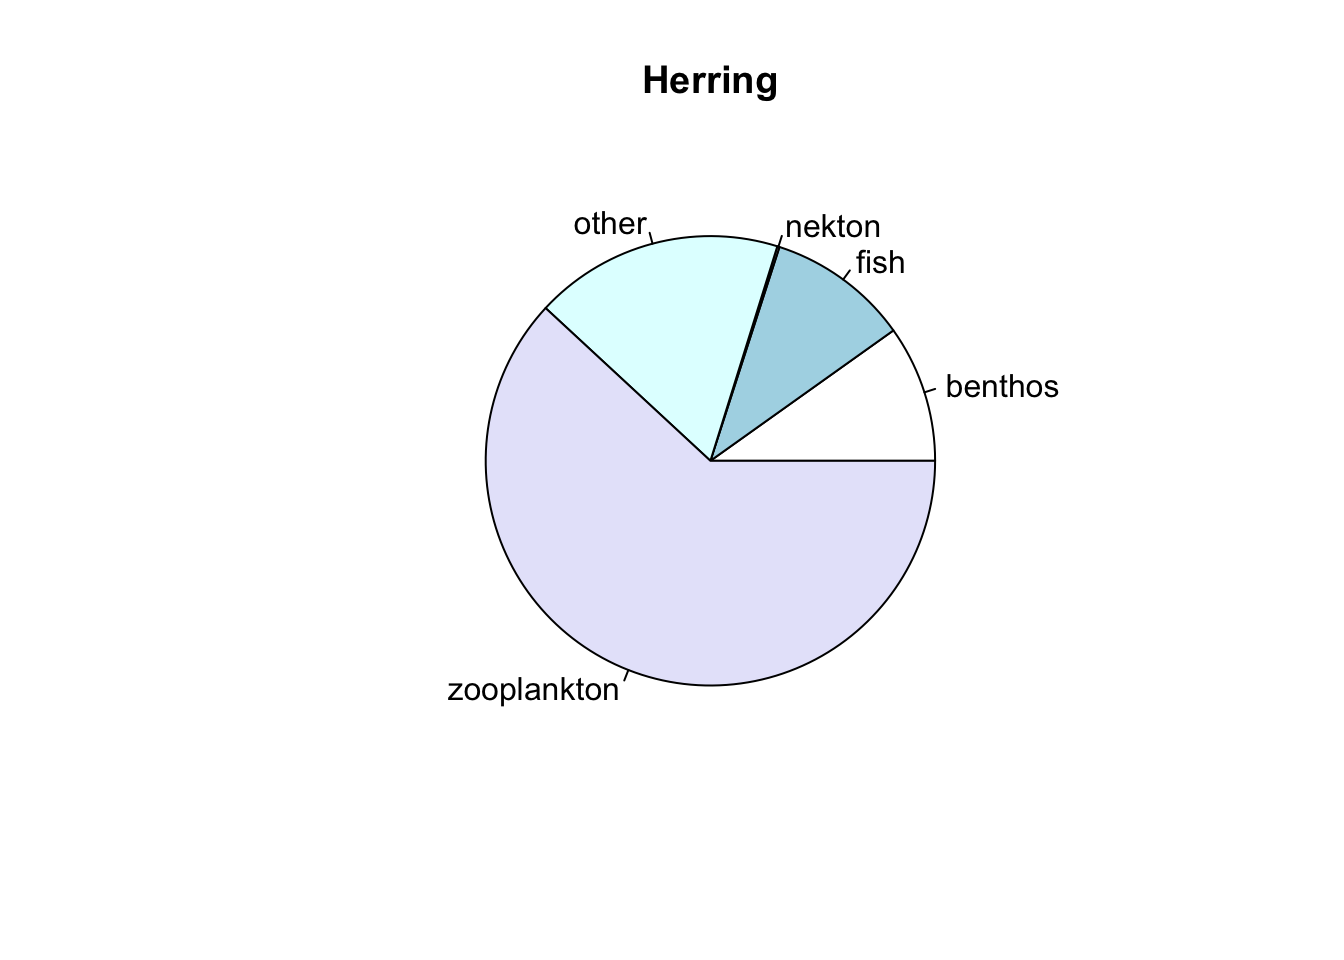
\includegraphics{Trials_files/figure-latex/distribution of prey-1.pdf}

\begin{Shaded}
\begin{Highlighting}[]
\CommentTok{\#geom\_bar() creates a bar chart from the specified data}
\CommentTok{\#facet\_wrap() means an individual bar chart is created for each individual predator species}
\CommentTok{\#\textquotesingle{}theme()\textquotesingle{} removes any words on the x{-}axis so the graphs are easier to understand}
\CommentTok{\#scale\_fill\_brewer changes the colour palette of the plot so that the colours are easy to distinguish between}
\end{Highlighting}
\end{Shaded}

These are individual bar charts showing the distribution of the type of
prey each predator eats.

The prey types are:

\begin{itemize}
\tightlist
\item
  Benthos: organisms that live on/near the bottom of a body of water
\item
  Fish: aquatic, craniate (have a skull), gill-bearing animals that lack
  limbs with digits (i.e.~their limbs don't have toes or fingers)
\item
  Nekton: the actively swimming aquatic organisms
\item
  Other: misc. types that don't fit into the other categories
\item
  Zooplankton: animal plankton (plankton are aquatic organisms that are
  unable to swim effectively against currents)
\end{itemize}

We can see that some predators eat a range of prey types (e.g.~Whiting),
while others prefer to eat a single prey type in abundance
(e.g.~European Hake and Monkfish mostly consume fish as their prey).

\hypertarget{most-common-prey-weights}{%
\section{Most common prey weights}\label{most-common-prey-weights}}

\begin{Shaded}
\begin{Highlighting}[]
\FunctionTok{ggplot}\NormalTok{(}\AttributeTok{data =}\NormalTok{ renamed\_df, }\FunctionTok{aes}\NormalTok{(lprey\_weight, no.\_prey\_per\_stmch)) }\SpecialCharTok{+} 
      \FunctionTok{labs}\NormalTok{(}\AttributeTok{title =} \StringTok{"log(prey weight) v. number of prey per predator stomach"}\NormalTok{, }
       \AttributeTok{x=}\StringTok{"log(prey weight)"}\NormalTok{, }\AttributeTok{y=}\StringTok{"No. of prey per predator stomach"}\NormalTok{) }\SpecialCharTok{+} 
      \FunctionTok{geom\_point}\NormalTok{(}\AttributeTok{size=}\FloatTok{0.5}\NormalTok{)}
\end{Highlighting}
\end{Shaded}

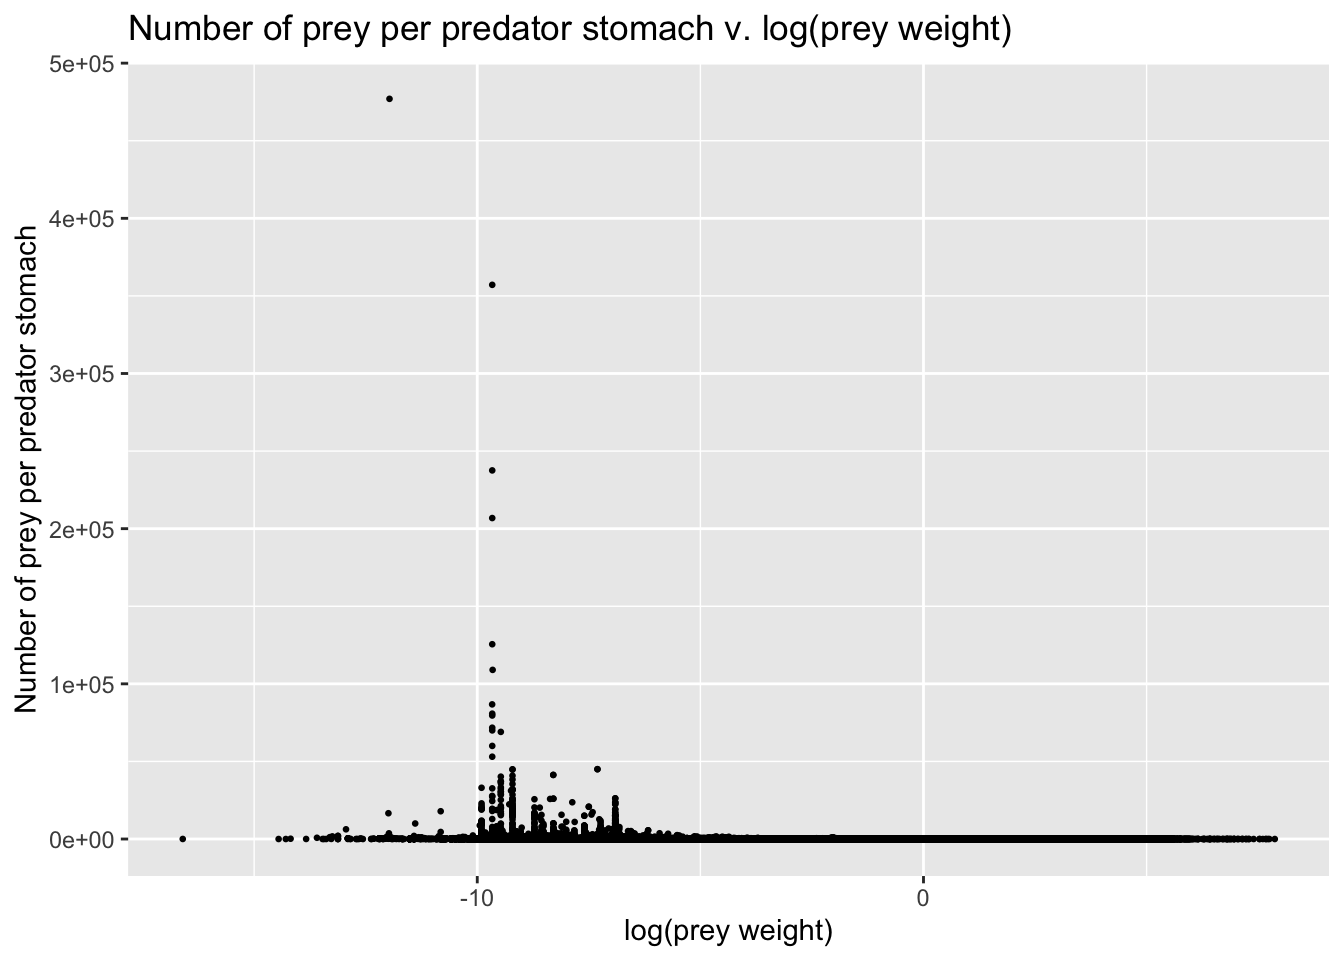
\includegraphics{Trials_files/figure-latex/log(prey weight) v. number of prey per stomach-1.pdf}

\begin{Shaded}
\begin{Highlighting}[]
\CommentTok{\#geom\_point() adds individual points which show individual recorded points}
\CommentTok{\#size=0.5 defines the size of each point on this graph}
\end{Highlighting}
\end{Shaded}

This graph is looking at the distribution of the weight of prey
recorded, i.e.~looking at what is the most common prey weight over all
prey species. It is a graph over all the data points, so includes
recordings from all the ships involved.

There are some potentially interesting results, so results from
different ships were plotted on individual curves to further look into
these results.

\begin{Shaded}
\begin{Highlighting}[]
\NormalTok{renamed\_df}\SpecialCharTok{$}\StringTok{\textquotesingle{}haul\_id\_short\textquotesingle{}} \OtherTok{\textless{}{-}} \FunctionTok{gsub}\NormalTok{(}\StringTok{"}\SpecialCharTok{\textbackslash{}\textbackslash{}}\StringTok{{-}.*"}\NormalTok{, }\StringTok{""}\NormalTok{, renamed\_df}\SpecialCharTok{$}\StringTok{\textquotesingle{}haul\_id\textquotesingle{}}\NormalTok{)}
\NormalTok{renamed\_df}\SpecialCharTok{$}\StringTok{\textquotesingle{}haul\_id\_short\textquotesingle{}} \OtherTok{\textless{}{-}} \FunctionTok{gsub}\NormalTok{(}\StringTok{"\_"}\NormalTok{, }\StringTok{""}\NormalTok{, renamed\_df}\SpecialCharTok{$}\StringTok{\textquotesingle{}haul\_id\_short\textquotesingle{}}\NormalTok{)}
\CommentTok{\#the haul\_id values are renamed to be shortened versions of the ship names (e.g. CLYDE) rather than the complete id (e.g. CLYDE{-}1935{-}6)}

\NormalTok{interesting\_haul }\OtherTok{\textless{}{-}} \FunctionTok{filter}\NormalTok{(renamed\_df, }
\NormalTok{                           haul\_id\_short}\SpecialCharTok{==}\StringTok{\textquotesingle{}CLYDE\textquotesingle{}}\SpecialCharTok{|}\NormalTok{haul\_id\_short}\SpecialCharTok{==}\StringTok{\textquotesingle{}END04\textquotesingle{}}\SpecialCharTok{|}\NormalTok{haul\_id\_short}\SpecialCharTok{==}\StringTok{\textquotesingle{}LUC\textquotesingle{}}\SpecialCharTok{|}
\NormalTok{                             haul\_id\_short}\SpecialCharTok{==}\StringTok{\textquotesingle{}HIDDINK\textquotesingle{}}\SpecialCharTok{|}\NormalTok{haul\_id\_short}\SpecialCharTok{==}\StringTok{\textquotesingle{}EXCmacDATSTO815\textquotesingle{}}\SpecialCharTok{|}
\NormalTok{                             haul\_id\_short}\SpecialCharTok{==}\StringTok{"Excmacdatsto815error"}\NormalTok{)}
\CommentTok{\#interesting\_haul is a new data frame which only contains values recorded by ships which gave "interesting" looking datapoints}

\NormalTok{haul\_list\_interesting }\OtherTok{\textless{}{-}} \FunctionTok{unique}\NormalTok{(interesting\_haul}\SpecialCharTok{$}\NormalTok{haul\_id\_short)}
\CommentTok{\#creates an array containing every individual (renamed) ship name that we are interested in}

\FunctionTok{ggplot}\NormalTok{ (}\AttributeTok{data =}\NormalTok{ interesting\_haul, }\FunctionTok{aes}\NormalTok{(}\AttributeTok{x=}\NormalTok{lprey\_weight, }\AttributeTok{y=}\NormalTok{no.\_prey\_per\_stmch)) }\SpecialCharTok{+} 
  \FunctionTok{labs}\NormalTok{(}\AttributeTok{title =} \StringTok{"log(prey weight) v. number of prey per stomach {-} separated by ship names"}\NormalTok{,}
       \AttributeTok{x=}\StringTok{"log(prey weight)"}\NormalTok{, }\AttributeTok{y=}\StringTok{"No. prey per stomach"}\NormalTok{) }\SpecialCharTok{+} 
  \FunctionTok{geom\_point}\NormalTok{(}\AttributeTok{size=}\FloatTok{0.02}\NormalTok{, }\AttributeTok{colour=}\StringTok{"red"}\NormalTok{) }\SpecialCharTok{+}
  \FunctionTok{theme}\NormalTok{(}\AttributeTok{strip.text =} \FunctionTok{element\_text}\NormalTok{(}\AttributeTok{size =} \DecValTok{5}\NormalTok{)) }\SpecialCharTok{+} 
  \FunctionTok{facet\_wrap}\NormalTok{(}\SpecialCharTok{\textasciitilde{}}\NormalTok{interesting\_haul}\SpecialCharTok{$}\NormalTok{haul\_id\_short, }\AttributeTok{scale=}\StringTok{"free\_y"}\NormalTok{)}
\end{Highlighting}
\end{Shaded}

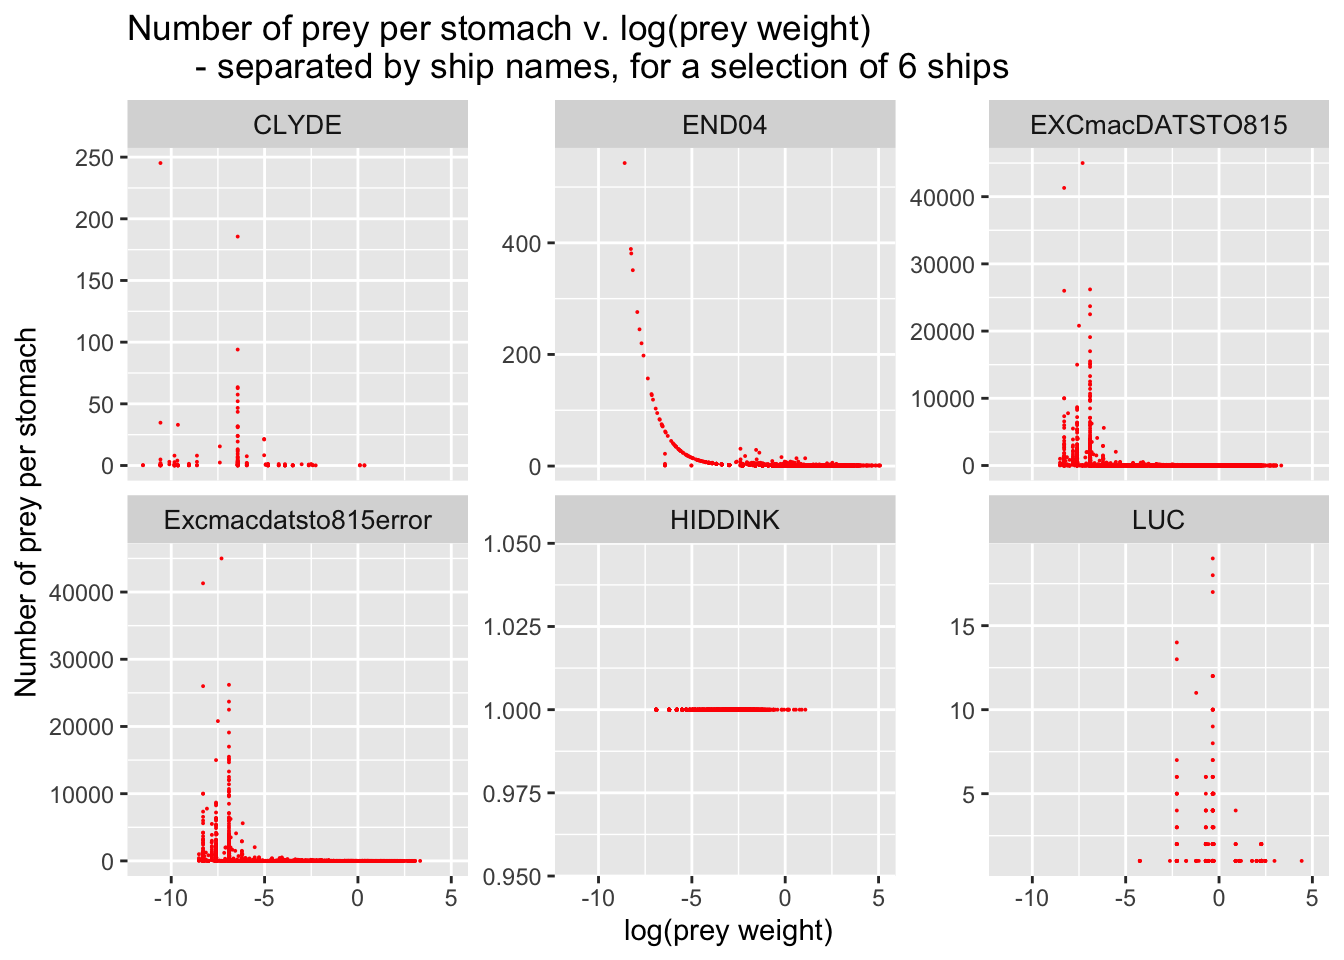
\includegraphics{Trials_files/figure-latex/sep by ships-1.pdf}

These six graphs show a range of unusual looking points:

\begin{enumerate}
\def\labelenumi{\arabic{enumi}.}
\tightlist
\item
  \(y \propto e^{-x}\) relation for END04 (i.e.~no. per stomach is
  proportional to 1/prey weight)
\item
  lots of observations for single prey weights for LUC and CLYDE
\item
  lots of the same no. of prey per stomach observations for HIDDINK.
\item
  the EXCmacDATSTO815 and Excmacdatsto815error seem to represent exactly
  the same data
\end{enumerate}

Though we will not remove or alter the data set to account for these
potentially erroneous data points in this project, for further analysis
it may be sensible to remove the data points these six ships recorded so
that final analysis is as reliable as possible.

\hypertarget{prey-and-predator-weight-relation}{%
\section{Prey and predator weight
relation}\label{prey-and-predator-weight-relation}}

\begin{Shaded}
\begin{Highlighting}[]
\CommentTok{\#message=FALSE means some output messages aren\textquotesingle{}t printed in the knitted HTML document}

\FunctionTok{ggplot}\NormalTok{(}\AttributeTok{data =}\NormalTok{ renamed\_df, }\FunctionTok{aes}\NormalTok{(lprey\_weight, lpred\_weight)) }\SpecialCharTok{+} 
  \FunctionTok{labs}\NormalTok{(}\AttributeTok{title =} \StringTok{"log(Predator mass) v. log(prey mass) plot"}\NormalTok{, }
       \AttributeTok{x=}\StringTok{"log(Prey mass)"}\NormalTok{, }\AttributeTok{y=}\StringTok{"log(Predator mass)"}\NormalTok{) }\SpecialCharTok{+} 
  \FunctionTok{geom\_hex}\NormalTok{(}\AttributeTok{bins =} \DecValTok{50}\NormalTok{) }\SpecialCharTok{+}
  \FunctionTok{scale\_fill\_gradient2}\NormalTok{(}\AttributeTok{low =} \StringTok{"black"}\NormalTok{, }\AttributeTok{mid=}\StringTok{"orange"}\NormalTok{, }\AttributeTok{high =} \StringTok{"red"}\NormalTok{, }\AttributeTok{midpoint=}\DecValTok{600}\NormalTok{) }\SpecialCharTok{+}
  \FunctionTok{stat\_smooth}\NormalTok{(}\AttributeTok{method=}\StringTok{\textquotesingle{}lm\textquotesingle{}}\NormalTok{, }\AttributeTok{se=}\ConstantTok{FALSE}\NormalTok{, }\AttributeTok{colour=}\StringTok{"blue"}\NormalTok{)}
\end{Highlighting}
\end{Shaded}

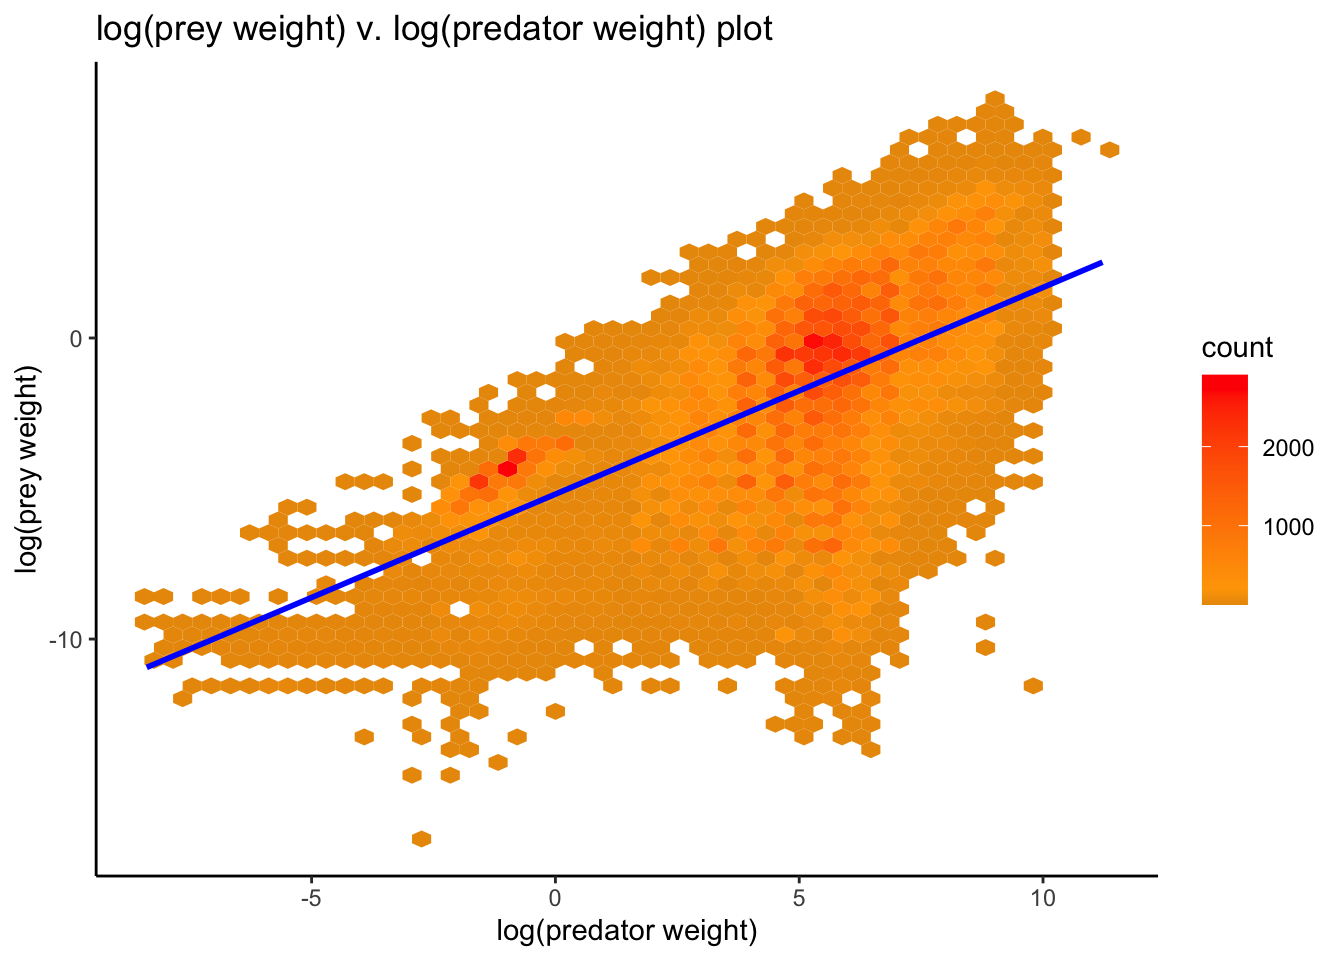
\includegraphics{Trials_files/figure-latex/log(prey weight) v. log(pred weight)-1.pdf}

\begin{Shaded}
\begin{Highlighting}[]
\CommentTok{\# stat\_smooth adds a line of best fit plotted through the points}
\CommentTok{\# method=\textquotesingle{}lm\textquotesingle{} ensures it is a straight line, i.e. a linear model}
\CommentTok{\# se=FAlSE creates only a single line, with no error of margin included}

\CommentTok{\#geom\_hex creates "bins" in the data where the density is calculated over}
\CommentTok{\#bins=50 means that there are 50 "bins" in the horizontal direction and 50 in the vertical}
\CommentTok{\#scale\_fill\_gradient2 creates a density colour scale, meaning that areas with a high density of points are red and areas with a low density of points are darker in colour}

\NormalTok{slope }\OtherTok{\textless{}{-}} \FunctionTok{coef}\NormalTok{(}\FunctionTok{lm}\NormalTok{(renamed\_df}\SpecialCharTok{$}\NormalTok{lpred\_weight}\SpecialCharTok{\textasciitilde{}}\NormalTok{renamed\_df}\SpecialCharTok{$}\NormalTok{lprey\_weight))}
\FunctionTok{paste}\NormalTok{(}\StringTok{"slope of the log(pred) v. log(prey) line of best fit:"}\NormalTok{, slope[}\DecValTok{2}\NormalTok{])}
\end{Highlighting}
\end{Shaded}

\begin{verbatim}
## [1] "slope of the log(pred) v. log(prey) line of best fit: 0.489336522809739"
\end{verbatim}

\begin{Shaded}
\begin{Highlighting}[]
\CommentTok{\# coef(lm()) creates an array containing the coefficients of the linear model of the relationship between two axes}
\CommentTok{\# The first item of the array gives out the y{-}intercept of the line, and the second item of the array is the gradient}
\end{Highlighting}
\end{Shaded}

We are attempting to find a link between the predator mass and the prey
mass. Log() of each axis is used to see the proportionality of the axes,
where the slope of the added line should = 1. This is because:

\[
 \log (\text{pred weight}) = m \times \text{log(prey weight)} + c
\]

Where m is the gradient of the slope and c is the y-intercept (thinking
of this graph as a linear model).

Taking the exponential of both sides,

\[
  \text{pred weight} = \exp({{m}\times{\log(\text{prey weight})}}) + \log(D)
\] where log(D) = c.~

Finally,

\[
  \text{pred weight} = \text{prey weight}^m \times D
\]

Hence, we want m=1 to show that pred weight proportional to prey weight
(as expected).

For this graph, the slope is not equal to one. However, this graph is
plotted over the entire data set and includes values from all of the
available predator species.

Instead, separate the plots by predator species to see if there is some
proportionality between the predator and prey weight for each specific
species.

\hypertarget{predator-v.-prey-weight-plot-separated-by-predator-species}{%
\subsection{Predator v. prey weight plot, separated by predator
species}\label{predator-v.-prey-weight-plot-separated-by-predator-species}}

\begin{Shaded}
\begin{Highlighting}[]
\FunctionTok{ggplot}\NormalTok{(}\AttributeTok{data =}\NormalTok{ renamed\_df, }\FunctionTok{aes}\NormalTok{(lprey\_weight, lpred\_weight)) }\SpecialCharTok{+} 
  \FunctionTok{labs}\NormalTok{(}\AttributeTok{title =} \StringTok{"log(pred. mass) v. log(prey mass) separated by predator species"}\NormalTok{, }
       \AttributeTok{x=}\StringTok{"log(prey mass)"}\NormalTok{, }\AttributeTok{y=}\StringTok{"log(pred. mass)"}\NormalTok{) }\SpecialCharTok{+}
  \FunctionTok{geom\_point}\NormalTok{(}\AttributeTok{size=}\FloatTok{0.2}\NormalTok{) }\SpecialCharTok{+} 
  \FunctionTok{facet\_wrap}\NormalTok{(}\SpecialCharTok{\textasciitilde{}}\NormalTok{pred\_species, }\AttributeTok{scale=}\StringTok{"free\_y"}\NormalTok{) }\SpecialCharTok{+} 
  \FunctionTok{theme}\NormalTok{(}\AttributeTok{strip.text =} \FunctionTok{element\_text}\NormalTok{(}\AttributeTok{size =} \DecValTok{10}\NormalTok{)) }\SpecialCharTok{+}
  \FunctionTok{stat\_smooth}\NormalTok{ (}\AttributeTok{method=}\StringTok{\textquotesingle{}lm\textquotesingle{}}\NormalTok{, }\AttributeTok{se=}\ConstantTok{FALSE}\NormalTok{, }\AttributeTok{colour=}\StringTok{"red"}\NormalTok{)}
\end{Highlighting}
\end{Shaded}

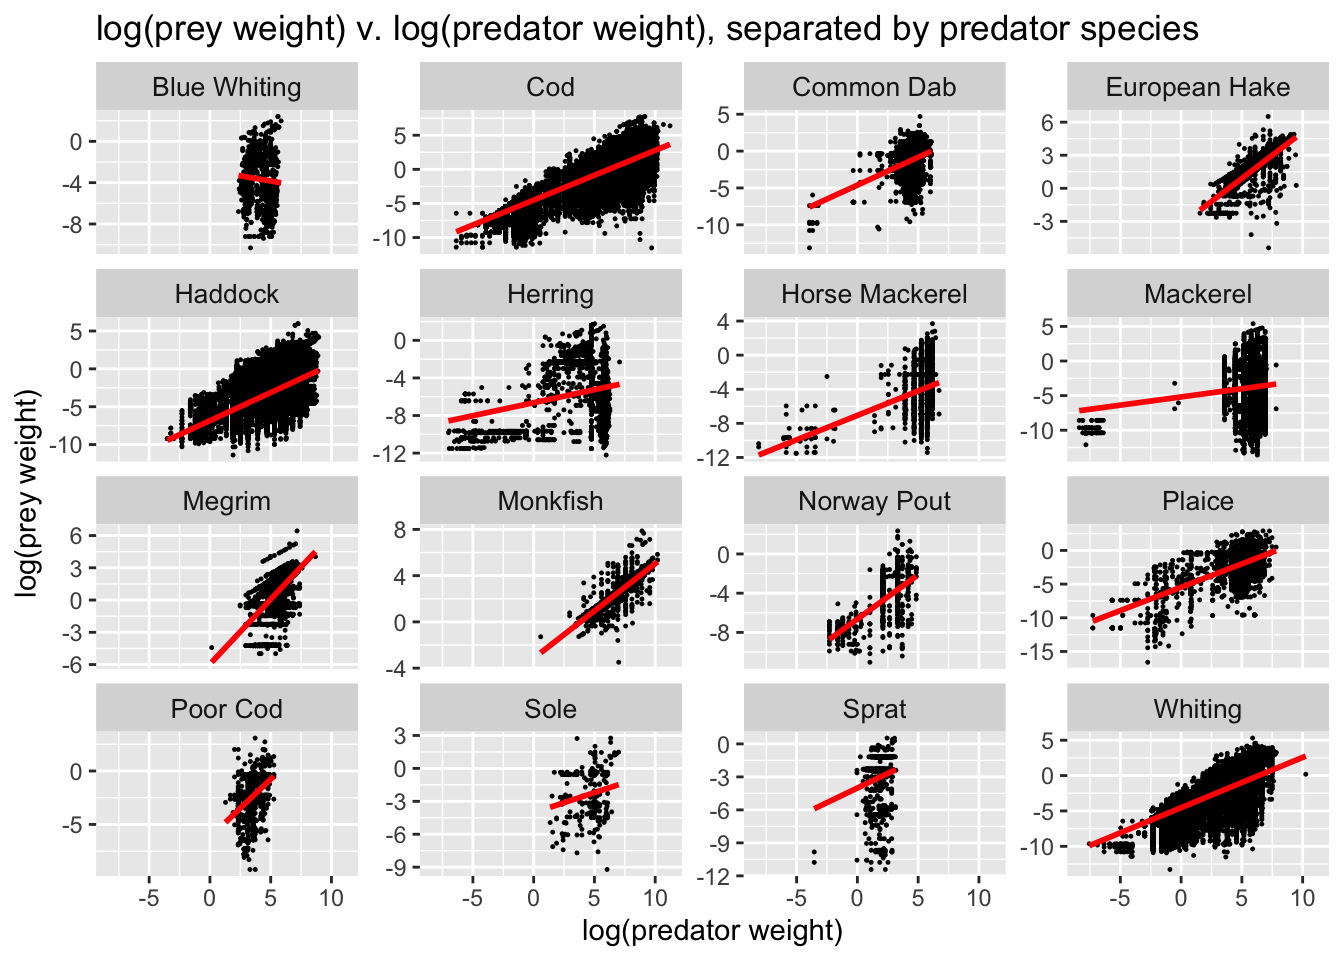
\includegraphics{Trials_files/figure-latex/sep by pred species-1.pdf}

\hypertarget{gradients-of-the-plots-for-each-predator-species}{%
\subsection{Gradients of the plots for each predator
species}\label{gradients-of-the-plots-for-each-predator-species}}

\begin{Shaded}
\begin{Highlighting}[]
\NormalTok{i }\OtherTok{\textless{}{-}} \DecValTok{1}
\NormalTok{species\_grad }\OtherTok{=} \FunctionTok{c}\NormalTok{()}
\CommentTok{\#setting i=1 for the while loop}
\CommentTok{\#and creating an empty vector called \textquotesingle{}species\_grad\textquotesingle{} to hold data}

\ControlFlowTok{while}\NormalTok{(i}\SpecialCharTok{\textless{}=}\FunctionTok{length}\NormalTok{(species\_list))\{}
\NormalTok{  species\_df }\OtherTok{\textless{}{-}}\NormalTok{ renamed\_df }\SpecialCharTok{\%\textgreater{}\%} \FunctionTok{filter}\NormalTok{(pred\_species }\SpecialCharTok{==} \FunctionTok{fixed}\NormalTok{(species\_list[i]))}
\NormalTok{  grad }\OtherTok{\textless{}{-}} \FunctionTok{coef}\NormalTok{(}\FunctionTok{lm}\NormalTok{((species\_df}\SpecialCharTok{$}\NormalTok{lpred\_weight)}\SpecialCharTok{\textasciitilde{}}\NormalTok{(species\_df}\SpecialCharTok{$}\NormalTok{lprey\_weight)))}
\NormalTok{  species\_grad[i] }\OtherTok{\textless{}{-}}\NormalTok{ grad[}\DecValTok{2}\NormalTok{]}
\NormalTok{  i}\OtherTok{=}\NormalTok{i}\SpecialCharTok{+}\DecValTok{1}
\NormalTok{\}}

\CommentTok{\#\textquotesingle{}while\textquotesingle{} means that this function repeats through the length of \textquotesingle{}species\_list\textquotesingle{} until all predator species are accounted for}
\CommentTok{\#i=i+1 increases the value of i each time through this loop to motivate this repeat}
\CommentTok{\#this creates a data frame (species\_df) containing each indivdual predator species, then calculates the gradient of the log(pred weight) v. log(prey weight) graph for this individual predator species, then inserts this gradient value to the ith value of an array named \textquotesingle{}species\_grad\textquotesingle{}}

\NormalTok{pvp\_grads }\OtherTok{\textless{}{-}} \FunctionTok{data.frame}\NormalTok{(}\AttributeTok{pred\_species=}\FunctionTok{c}\NormalTok{(species\_list),}
                        \AttributeTok{gradient=}\FunctionTok{c}\NormalTok{(species\_grad))}

\FunctionTok{kable}\NormalTok{(pvp\_grads)}
\end{Highlighting}
\end{Shaded}

\begin{longtable}[]{@{}lr@{}}
\toprule()
pred\_species & gradient \\
\midrule()
\endhead
Blue Whiting & -0.0258049 \\
Cod & 0.8343249 \\
Common Dab & 0.1217269 \\
European Hake & 0.7230261 \\
Haddock & 0.2604050 \\
Herring & 0.2220153 \\
Horse Mackerel & 0.2290883 \\
Mackerel & 0.0156493 \\
Megrim & 0.3020678 \\
Monkfish & 0.7009350 \\
Norway Pout & 0.4455201 \\
Plaice & 0.4548590 \\
Poor Cod & 0.1394437 \\
Sole & 0.1141953 \\
Sprat & 0.0381477 \\
Whiting & 0.6664210 \\
\bottomrule()
\end{longtable}

\begin{Shaded}
\begin{Highlighting}[]
\CommentTok{\#creates a new data frame name \textquotesingle{}pvp\_grads\textquotesingle{}, with one column named \textquotesingle{}pred\_species\textquotesingle{} and the other named \textquotesingle{}gradient\textquotesingle{}}
\CommentTok{\#each row contains the name of some individual predator species and its associated gradient}
\CommentTok{\#kable prints the information in the pvp\_grads}
\end{Highlighting}
\end{Shaded}

Here, we are splitting up the graphs over each individual predator
species to look and see if there is a proportionality for each specific
species.

We are wanting gradient=1 for proportionality. This is only true (to 1
significant figure) for the species Cod, European Hake, Monkfish and
Whiting. Although this is a very limited number of the predator species,
the assumption that the predator and prey masses are proportional is a
reasonable one, so we will continue wiht this assumption.

\hypertarget{predator-weight-against-ppmr}{%
\section{Predator weight against
ppmr}\label{predator-weight-against-ppmr}}

\hypertarget{plotting-predator-weight-against-ppmr-separated-by-predator-species}{%
\subsection{Plotting predator weight against ppmr, separated by predator
species}\label{plotting-predator-weight-against-ppmr-separated-by-predator-species}}

\begin{Shaded}
\begin{Highlighting}[]
\FunctionTok{ggplot}\NormalTok{(}\AttributeTok{data=}\NormalTok{renamed\_df, }\FunctionTok{aes}\NormalTok{(lpred\_weight, lppmr)) }\SpecialCharTok{+} 
  \FunctionTok{geom\_point}\NormalTok{(}\AttributeTok{size=}\FloatTok{0.001}\NormalTok{) }\SpecialCharTok{+}
  \FunctionTok{labs}\NormalTok{(}\AttributeTok{title =} \StringTok{"log(pred mass) v. log(ppmr) plot"}\NormalTok{, }\AttributeTok{x=}\StringTok{"log(Pred mass)"}\NormalTok{, }\AttributeTok{y=}\StringTok{"log(PPMR)"}\NormalTok{) }\SpecialCharTok{+} 
  \FunctionTok{stat\_smooth}\NormalTok{ (}\AttributeTok{method=}\StringTok{\textquotesingle{}lm\textquotesingle{}}\NormalTok{, }\AttributeTok{se=}\ConstantTok{FALSE}\NormalTok{) }\SpecialCharTok{+} 
  \FunctionTok{facet\_wrap}\NormalTok{(}\SpecialCharTok{\textasciitilde{}}\NormalTok{pred\_species, }\AttributeTok{scale=}\StringTok{"free\_y"}\NormalTok{)}
\end{Highlighting}
\end{Shaded}

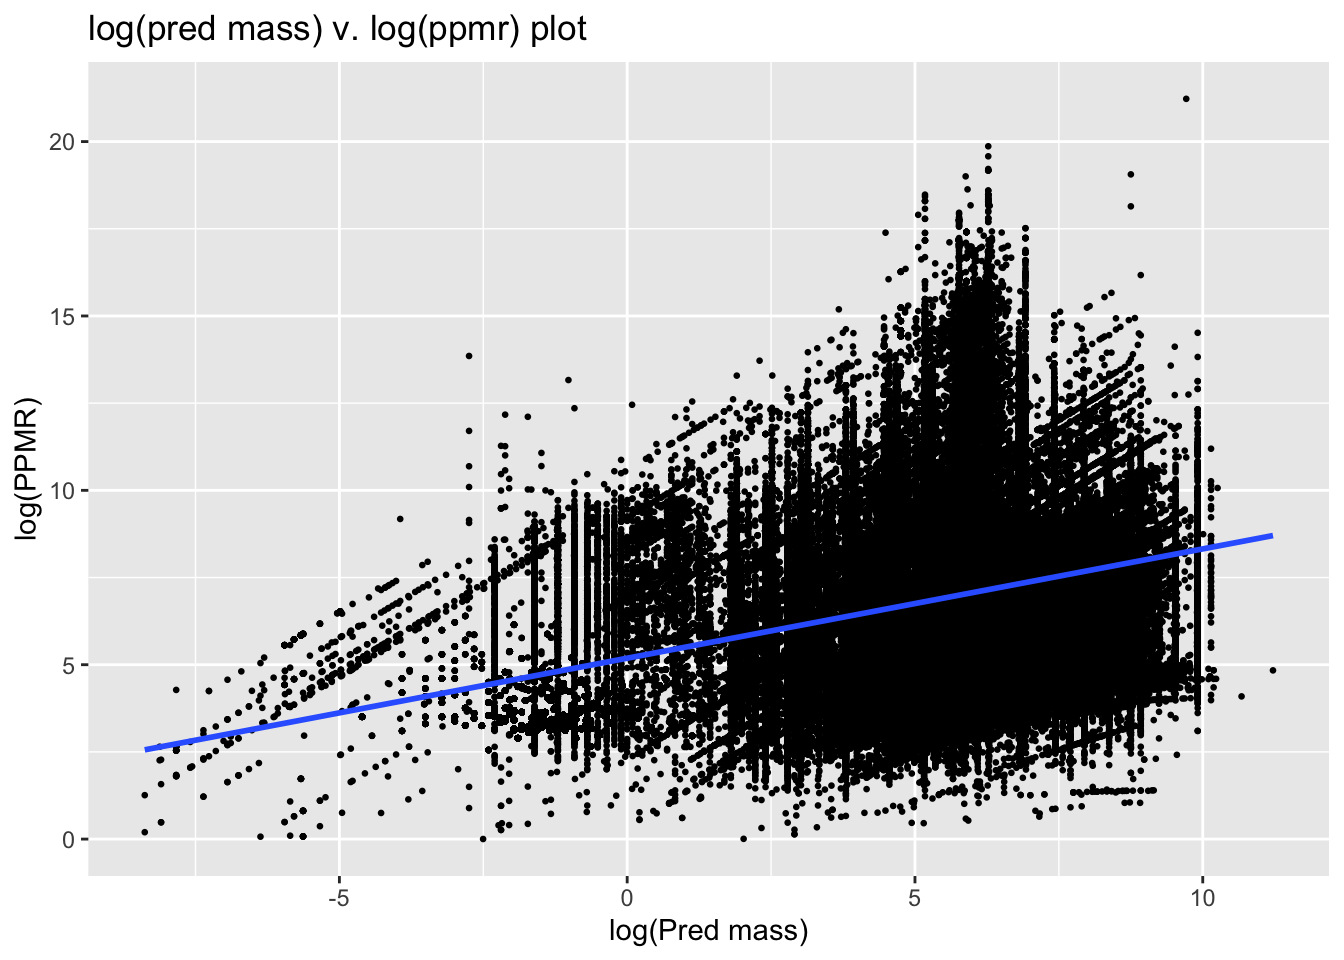
\includegraphics{Trials_files/figure-latex/pred weight v. ppmr-1.pdf}

Graphing log(pred mass) v. log(ppmr) for individual predator species to
see if the predator mass related to the ppmr.

\[
    \log(\text{pred mass}) = m \times \log (\text{prey mass}) + c
\]

where m is the gradient (assuming a linear model between the variables)
and c is the y-intercept.

We want them to not be proportional (i.e.~slope, m= 0) to prove that
log(predator mass) is not related to the log(ppmr) (and hence the ppmr
is independent of the predator mass for a certain species).

\hypertarget{gradients-of-the-plots}{%
\subsection{Gradients of the plots}\label{gradients-of-the-plots}}

\begin{Shaded}
\begin{Highlighting}[]
\NormalTok{species\_grad\_ppmr}\OtherTok{=}\FunctionTok{c}\NormalTok{()}
\NormalTok{j }\OtherTok{\textless{}{-}} \DecValTok{1}
\CommentTok{\#creates an empty vector called \textquotesingle{}species\_grad\_ppmr\textquotesingle{}}
\CommentTok{\#setting j=1 for the while loop}

\ControlFlowTok{while}\NormalTok{(j}\SpecialCharTok{\textless{}=}\FunctionTok{length}\NormalTok{(species\_list))\{}
\NormalTok{  species\_df }\OtherTok{\textless{}{-}}\NormalTok{ renamed\_df }\SpecialCharTok{\%\textgreater{}\%} \FunctionTok{filter}\NormalTok{(pred\_species }\SpecialCharTok{==} \FunctionTok{fixed}\NormalTok{(species\_list[j]))}
\NormalTok{  grad }\OtherTok{\textless{}{-}} \FunctionTok{coef}\NormalTok{(}\FunctionTok{lm}\NormalTok{((species\_df}\SpecialCharTok{$}\NormalTok{lppmr)}\SpecialCharTok{\textasciitilde{}}\NormalTok{(species\_df}\SpecialCharTok{$}\NormalTok{lpred\_weight)))}
\NormalTok{  species\_grad\_ppmr[j] }\OtherTok{\textless{}{-}}\NormalTok{ grad[}\DecValTok{2}\NormalTok{]}
\NormalTok{  j}\OtherTok{=}\NormalTok{j}\SpecialCharTok{+}\DecValTok{1}
\NormalTok{\}}

\NormalTok{ppmrvp\_grads }\OtherTok{\textless{}{-}} \FunctionTok{data.frame}\NormalTok{(}\AttributeTok{pred\_species=}\FunctionTok{c}\NormalTok{(species\_list),}
                        \AttributeTok{gradient=}\FunctionTok{c}\NormalTok{(species\_grad\_ppmr))}

\FunctionTok{kable}\NormalTok{(ppmrvp\_grads)}
\end{Highlighting}
\end{Shaded}

\begin{longtable}[]{@{}lr@{}}
\toprule()
pred\_species & gradient \\
\midrule()
\endhead
Blue Whiting & 1.2032364 \\
Cod & 0.2709018 \\
Common Dab & 0.2435919 \\
European Hake & 0.1617011 \\
Haddock & 0.2581471 \\
Herring & 0.7232217 \\
Horse Mackerel & 0.4273000 \\
Mackerel & 0.7621392 \\
Megrim & -0.2055083 \\
Monkfish & 0.1811160 \\
Norway Pout & 0.0973909 \\
Plaice & 0.3061335 \\
Poor Cod & -0.0895529 \\
Sole & 0.6335299 \\
Sprat & 0.4688564 \\
Whiting & 0.2891959 \\
\bottomrule()
\end{longtable}

For the assumption to be upheld, we need gradient=0. This is
(approximately) satisfied for the species Cod, Common Dab, Euorpean
Hake, Haddock, Megrim, Monkfish, Norway Pout and Poor Cod. Although none
of these are exactly equal to 0, they are sufficiently close to continue
with the assumption that the ppmr is independent of the predator mass
for the named predator species.

\hypertarget{different-weightings}{%
\subsection{Different weightings}\label{different-weightings}}

\begin{Shaded}
\begin{Highlighting}[]
\NormalTok{species\_df }\OtherTok{\textless{}{-}}\NormalTok{ renamed\_df }\SpecialCharTok{\%\textgreater{}\%} \FunctionTok{filter}\NormalTok{(pred\_species }\SpecialCharTok{==} \FunctionTok{fixed}\NormalTok{(}\StringTok{"Poor Cod"}\NormalTok{))}
\CommentTok{\#creating a data frame only containing observations where the predator species is poor cod.}

\FunctionTok{ggplot}\NormalTok{(}\AttributeTok{data=}\NormalTok{species\_df, }\FunctionTok{aes}\NormalTok{(lpred\_weight, lppmr)) }\SpecialCharTok{+} 
  \FunctionTok{geom\_point}\NormalTok{(}\AttributeTok{size=}\FloatTok{0.5}\NormalTok{) }\SpecialCharTok{+}
  \FunctionTok{labs}\NormalTok{(}\AttributeTok{title =} \StringTok{"log(pred mass) v. log(ppmr) plot: Poor Cod"}\NormalTok{, }\AttributeTok{x=}\StringTok{"log(Pred mass)"}\NormalTok{, }\AttributeTok{y=}\StringTok{"log(PPMR)"}\NormalTok{) }\SpecialCharTok{+} 
  \FunctionTok{facet\_wrap}\NormalTok{(}\SpecialCharTok{\textasciitilde{}}\NormalTok{pred\_species, }\AttributeTok{scale=}\StringTok{"free\_y"}\NormalTok{) }\SpecialCharTok{+} 
  \FunctionTok{stat\_smooth}\NormalTok{(}\FunctionTok{aes}\NormalTok{(}\AttributeTok{weight=}\NormalTok{no.\_prey\_per\_stmch, }\AttributeTok{colour=}\StringTok{\textquotesingle{}by no. of prey in stomach\textquotesingle{}}\NormalTok{), }\AttributeTok{method=}\StringTok{\textquotesingle{}lm\textquotesingle{}}\NormalTok{, }\AttributeTok{se=}\ConstantTok{FALSE}\NormalTok{) }\SpecialCharTok{+}
  \FunctionTok{stat\_smooth}\NormalTok{(}\FunctionTok{aes}\NormalTok{(}\AttributeTok{colour=}\StringTok{\textquotesingle{}no weighting\textquotesingle{}}\NormalTok{), }\AttributeTok{method=}\StringTok{\textquotesingle{}lm\textquotesingle{}}\NormalTok{, }\AttributeTok{se=}\ConstantTok{FALSE}\NormalTok{) }\SpecialCharTok{+}
  \FunctionTok{stat\_smooth}\NormalTok{(}\FunctionTok{aes}\NormalTok{(}\AttributeTok{weight=}\NormalTok{prey\_weight\_g, }\AttributeTok{colour=}\StringTok{\textquotesingle{}by prey bio\textquotesingle{}}\NormalTok{), }\AttributeTok{method=}\StringTok{\textquotesingle{}lm\textquotesingle{}}\NormalTok{, }\AttributeTok{se=}\ConstantTok{FALSE}\NormalTok{) }\SpecialCharTok{+}
  \FunctionTok{stat\_summary}\NormalTok{(}\AttributeTok{fun.data=}\NormalTok{mean\_se, }\AttributeTok{geom=}\StringTok{"linerange"}\NormalTok{) }\SpecialCharTok{+}
  \FunctionTok{scale\_colour\_manual}\NormalTok{(}\AttributeTok{name=}\StringTok{"Weightings"}\NormalTok{,}
                     \AttributeTok{values=}\FunctionTok{c}\NormalTok{(}\StringTok{\textquotesingle{}by no. of prey in stomach\textquotesingle{}}\OtherTok{=}\StringTok{\textquotesingle{}blue\textquotesingle{}}\NormalTok{, }
                              \StringTok{\textquotesingle{}no weighting\textquotesingle{}}\OtherTok{=}\StringTok{\textquotesingle{}red\textquotesingle{}}\NormalTok{, }\StringTok{\textquotesingle{}by prey bio\textquotesingle{}}\OtherTok{=}\StringTok{\textquotesingle{}green\textquotesingle{}}\NormalTok{))}
\end{Highlighting}
\end{Shaded}

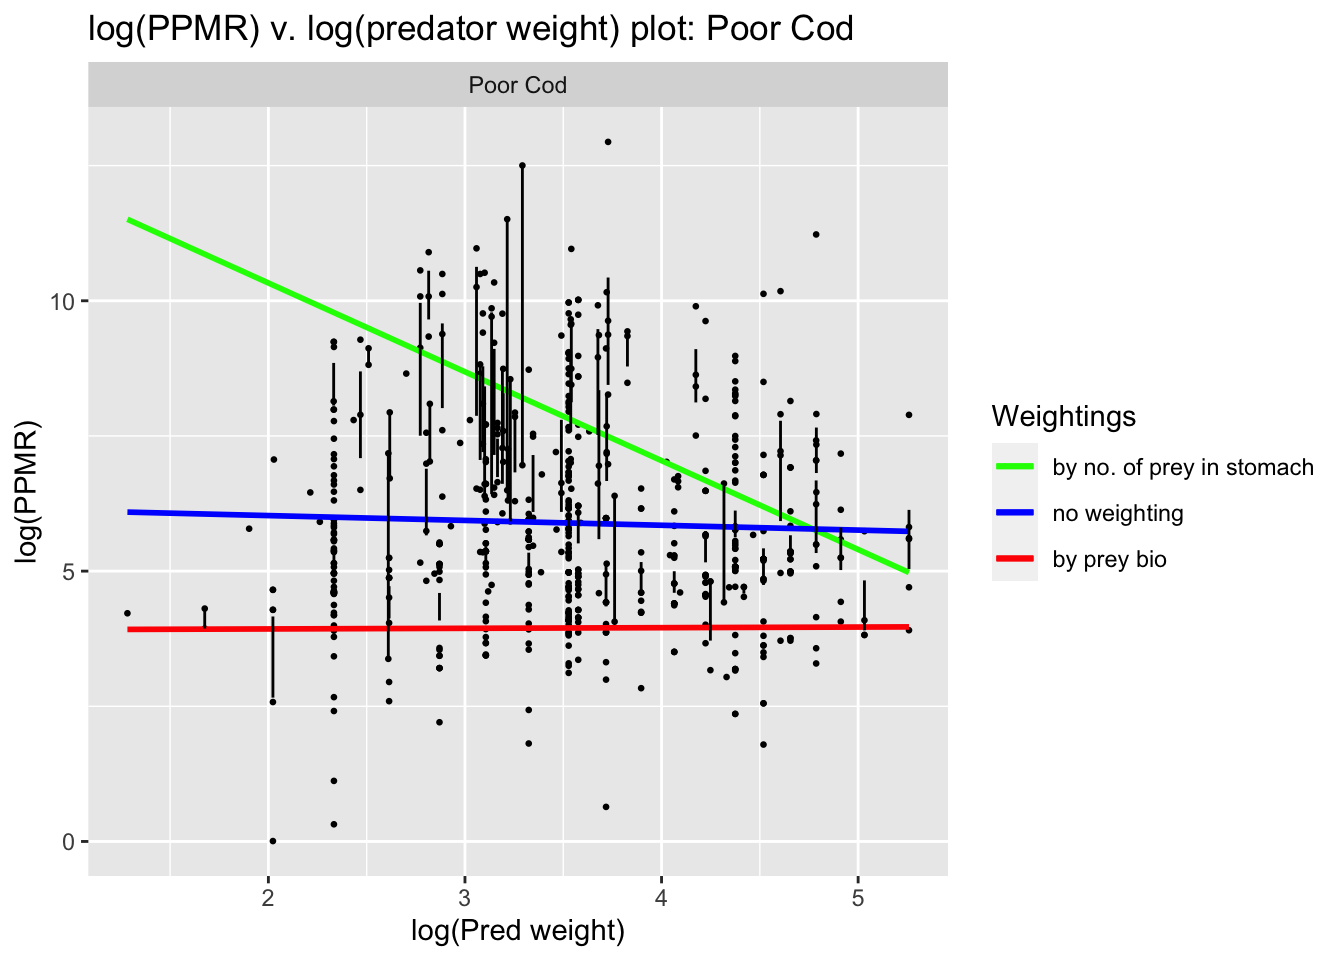
\includegraphics{Trials_files/figure-latex/poor cod-1.pdf}

\begin{Shaded}
\begin{Highlighting}[]
\CommentTok{\# se=FALSE doesn\textquotesingle{}t add an area of error around the LOBF }
\CommentTok{\# fun.data=mean\_se calculates the mean and standard error for each point}
\CommentTok{\# linerange draws a point range between an upper and lower limit for the line, and the mean for the point (using the values calcuated in \textquotesingle{}fun.data=mean\_se\textquotesingle{})}

\FunctionTok{paste}\NormalTok{(}\StringTok{"slope of the log(ppmr) v. log(pred\_weight) line of best fit for poor cod:"}\NormalTok{)}
\end{Highlighting}
\end{Shaded}

\begin{verbatim}
## [1] "slope of the log(ppmr) v. log(pred_weight) line of best fit for poor cod:"
\end{verbatim}

\begin{Shaded}
\begin{Highlighting}[]
\CommentTok{\#weighted by number of prey per stomach}
\NormalTok{perstmch\_weighting }\OtherTok{\textless{}{-}} 
  \FunctionTok{coef}\NormalTok{(}\FunctionTok{lm}\NormalTok{(species\_df}\SpecialCharTok{$}\NormalTok{lppmr}\SpecialCharTok{\textasciitilde{}}\NormalTok{species\_df}\SpecialCharTok{$}\NormalTok{lpred\_weight, }\AttributeTok{weight=}\NormalTok{species\_df}\SpecialCharTok{$}\NormalTok{no.\_prey\_per\_stmch))}
\FunctionTok{paste}\NormalTok{(}\StringTok{"i) Weighted by no prey in the stomach:"}\NormalTok{, perstmch\_weighting[}\DecValTok{2}\NormalTok{])}
\end{Highlighting}
\end{Shaded}

\begin{verbatim}
## [1] "i) Weighted by no prey in the stomach: -1.64313946193691"
\end{verbatim}

\begin{Shaded}
\begin{Highlighting}[]
\CommentTok{\#no weighting}
\NormalTok{no\_weighting }\OtherTok{\textless{}{-}} \FunctionTok{coef}\NormalTok{(}\FunctionTok{lm}\NormalTok{(species\_df}\SpecialCharTok{$}\NormalTok{lppmr}\SpecialCharTok{\textasciitilde{}}\NormalTok{species\_df}\SpecialCharTok{$}\NormalTok{lpred\_weight))}
\FunctionTok{paste}\NormalTok{(}\StringTok{"ii) No weighting in the calculation:"}\NormalTok{, no\_weighting[}\DecValTok{2}\NormalTok{])}
\end{Highlighting}
\end{Shaded}

\begin{verbatim}
## [1] "ii) No weighting in the calculation: -0.0895529388001952"
\end{verbatim}

\begin{Shaded}
\begin{Highlighting}[]
\CommentTok{\#weighted by prey biomass}
\NormalTok{biomass\_weighting }\OtherTok{\textless{}{-}} 
  \FunctionTok{coef}\NormalTok{(}\FunctionTok{lm}\NormalTok{(species\_df}\SpecialCharTok{$}\NormalTok{lppmr}\SpecialCharTok{\textasciitilde{}}\NormalTok{species\_df}\SpecialCharTok{$}\NormalTok{lpred\_weight, }\AttributeTok{weight=}\NormalTok{species\_df}\SpecialCharTok{$}\NormalTok{prey\_weight\_g))}
\FunctionTok{paste}\NormalTok{(}\StringTok{"iii) Weighted by prey biomass:"}\NormalTok{, biomass\_weighting[}\DecValTok{2}\NormalTok{])}
\end{Highlighting}
\end{Shaded}

\begin{verbatim}
## [1] "iii) Weighted by prey biomass: 0.0116668819369047"
\end{verbatim}

Looking at just the predator species `poor cod'. There are three LOBF
(line of best fit), weighted by different variables:

\begin{enumerate}
\def\labelenumi{\arabic{enumi}.}
\tightlist
\item
  blue: by number of prey per stomach
\item
  red: no weighting in the LOBF
\item
  green: by prey biomass
\end{enumerate}

When weighted by prey biomass, the gradient is equal to zero for 2 s.f..
Hence, the approximation (of slope=0) is true when looking at a prey
biomass weighting.

\hypertarget{average-ppmr-for-individual-species}{%
\section{Average PPMR for individual
species}\label{average-ppmr-for-individual-species}}

Here, we are looking for the most common log(PPMR) for each individual
species. This will be done by plotting log(PPMR) against the density of
points, and weighting observations on different variables. By assuming
these are normally distributed relations, there should be a `peak' point
of log(ppmr) which is where the mean/most common log(ppmr) value lies.
We assume this will be different for different species of predator,
i.e.~each predator has a preferred ppmr value and hence each predator
type has a preferred relative size of prey.

\hypertarget{weighted-by-prey-biomass}{%
\subsection{Weighted by prey biomass:}\label{weighted-by-prey-biomass}}

\begin{Shaded}
\begin{Highlighting}[]
\FunctionTok{ggplot}\NormalTok{(}\AttributeTok{data =}\NormalTok{ renamed\_df, }\FunctionTok{aes}\NormalTok{(}\AttributeTok{x=}\NormalTok{lppmr)) }\SpecialCharTok{+} 
  \FunctionTok{labs}\NormalTok{(}\AttributeTok{title =} \StringTok{"log(PPMR) v. biomass density of prey"}\NormalTok{, }\AttributeTok{x=}\StringTok{"log(PPMR)"}\NormalTok{, }\AttributeTok{y=}\StringTok{"Biomass density of prey"}\NormalTok{) }\SpecialCharTok{+}
  \FunctionTok{facet\_wrap}\NormalTok{(}\SpecialCharTok{\textasciitilde{}}\NormalTok{renamed\_df}\SpecialCharTok{$}\NormalTok{pred\_species, }\AttributeTok{scale=}\StringTok{"free\_y"}\NormalTok{) }\SpecialCharTok{+} 
  \FunctionTok{theme}\NormalTok{(}\AttributeTok{strip.text =} \FunctionTok{element\_text}\NormalTok{(}\AttributeTok{size =} \DecValTok{5}\NormalTok{)) }\SpecialCharTok{+}
  \FunctionTok{geom\_density}\NormalTok{(}\FunctionTok{aes}\NormalTok{(}\AttributeTok{weight =}\NormalTok{ prey\_weight\_g), }\AttributeTok{colour=}\StringTok{"red"}\NormalTok{)}
\end{Highlighting}
\end{Shaded}

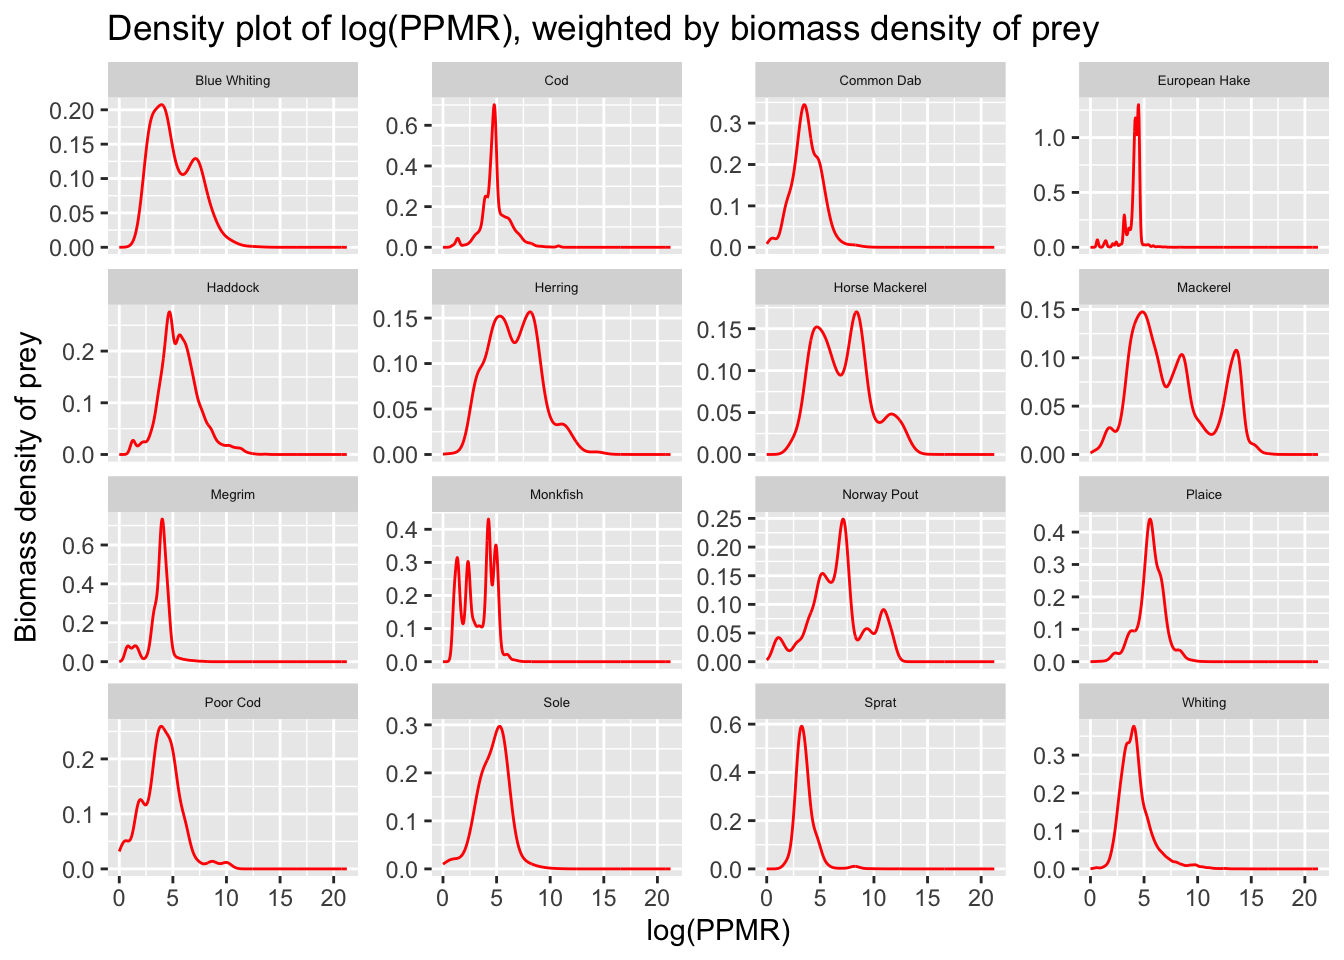
\includegraphics{Trials_files/figure-latex/ave PPMR biomass-1.pdf}

\begin{Shaded}
\begin{Highlighting}[]
\CommentTok{\#using facet\_wrap for the variable (pred\_species) means the data is separated into individual plots for each predator species}
\CommentTok{\#geom\_density means area under the curve = 1 (i.e. the graph is normalised)}
\CommentTok{\#weight=prey\_weight\_g means the points are \textquotesingle{}weighted\textquotesingle{} by the column weight (biomass) of each individual prey}
\end{Highlighting}
\end{Shaded}

These plots are weighted by the prey biomass. This means that we are
looking at the distribution of prey biomass across values of log(PPMR),
so points with a larger biomass are prioritised/weighted more than those
with a smaller biomass.

\hypertarget{weighted-by-number-of-prey}{%
\subsection{Weighted by number of
prey:}\label{weighted-by-number-of-prey}}

\begin{Shaded}
\begin{Highlighting}[]
\FunctionTok{ggplot}\NormalTok{(}\AttributeTok{data =}\NormalTok{ renamed\_df, }\FunctionTok{aes}\NormalTok{(}\AttributeTok{x=}\NormalTok{lppmr)) }\SpecialCharTok{+} 
  \FunctionTok{labs}\NormalTok{(}\AttributeTok{title =} \StringTok{"log(PPMR) v. number density of prey"}\NormalTok{, }\AttributeTok{x=}\StringTok{"log(PPMR)"}\NormalTok{, }\AttributeTok{y=}\StringTok{"Number density of prey"}\NormalTok{) }\SpecialCharTok{+}
  \FunctionTok{facet\_wrap}\NormalTok{(}\SpecialCharTok{\textasciitilde{}}\NormalTok{renamed\_df}\SpecialCharTok{$}\NormalTok{pred\_species, }\AttributeTok{scale=}\StringTok{"free\_y"}\NormalTok{) }\SpecialCharTok{+} 
  \FunctionTok{theme}\NormalTok{(}\AttributeTok{strip.text =} \FunctionTok{element\_text}\NormalTok{(}\AttributeTok{size =} \DecValTok{5}\NormalTok{)) }\SpecialCharTok{+}
  \FunctionTok{geom\_density}\NormalTok{(}\FunctionTok{aes}\NormalTok{(}\AttributeTok{weight =}\NormalTok{ no.\_prey\_per\_stmch), }\AttributeTok{colour=}\StringTok{"red"}\NormalTok{)}
\end{Highlighting}
\end{Shaded}

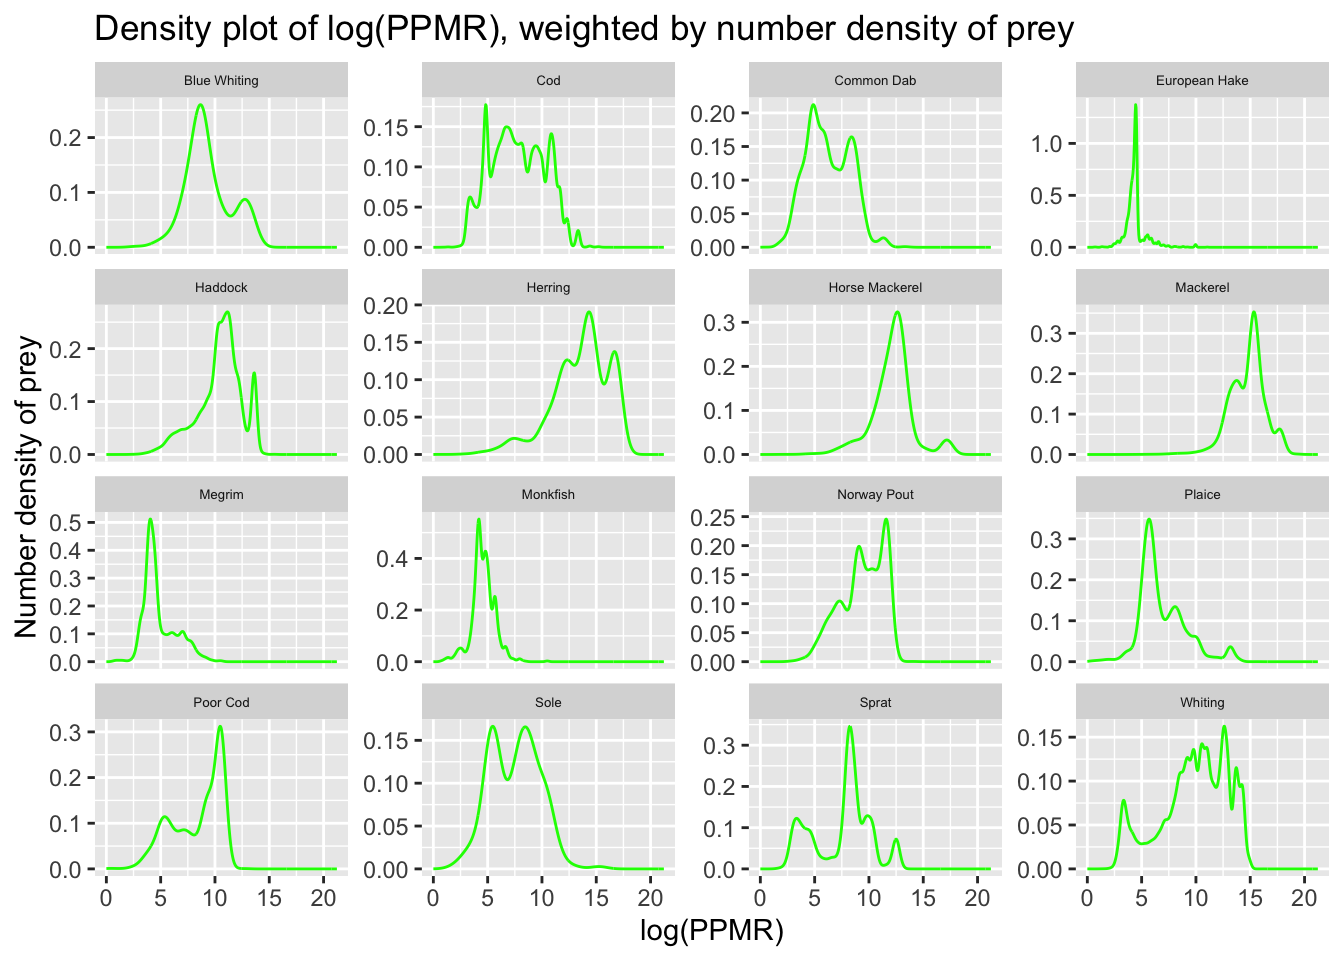
\includegraphics{Trials_files/figure-latex/ave PPMR prey no.-1.pdf}

\begin{Shaded}
\begin{Highlighting}[]
\CommentTok{\#weight=no.\_prey\_per\_stmch means the points are \textquotesingle{}weighted\textquotesingle{} by the number of prey per stomach}
\end{Highlighting}
\end{Shaded}

These plots are weighted by the number pf prey per stomach. This means
that data points with a larger number of prey per stomach are
prioritised/weighted more than those with a smaller number of prey per
stomach.

By looking at the two differently weighted graphs, it is clear to see
that the plots are `shifted' by some amount (e.g.~the Blue Whiting when
weighted by prey biomass has a mean log(ppmr) of roughly 4.8, and when
weighted by number of prey this mean becomes roughly 7.5).

\hypertarget{specific-ppmr-calculations-by-different-weightings-for-herring-species}{%
\section{Specific PPMR calculations by different weightings for Herring
species}\label{specific-ppmr-calculations-by-different-weightings-for-herring-species}}

Here, we take only observations relating to the predator type Herring.
This allows us to do more specific analysis about the shifted mean and
begin to explain some of the maths behind this shifting.

\begin{Shaded}
\begin{Highlighting}[]
\NormalTok{herringDF }\OtherTok{\textless{}{-}}\NormalTok{ renamed\_df }\SpecialCharTok{\%\textgreater{}\%} 
    \FunctionTok{filter}\NormalTok{(pred\_species }\SpecialCharTok{==} \FunctionTok{fixed}\NormalTok{(}\StringTok{"Herring"}\NormalTok{))}
\CommentTok{\#creates a separate data set (called \textquotesingle{}herringDF\textquotesingle{}) only containing observations for the predator species \textquotesingle{}Herring\textquotesingle{}}
\end{Highlighting}
\end{Shaded}

\hypertarget{weighted-by-prey-biomass-1}{%
\subsection{Weighted by prey biomass}\label{weighted-by-prey-biomass-1}}

\begin{Shaded}
\begin{Highlighting}[]
\NormalTok{bio\_herringmean }\OtherTok{=} \FunctionTok{weighted.mean}\NormalTok{(herringDF}\SpecialCharTok{$}\NormalTok{lppmr, }\AttributeTok{w =}\NormalTok{ herringDF}\SpecialCharTok{$}\NormalTok{prey\_weight\_g, }\AttributeTok{na.rm =} \ConstantTok{TRUE}\NormalTok{)}
\NormalTok{bio\_herringSD }\OtherTok{=} \FunctionTok{sqrt}\NormalTok{(}\FunctionTok{wtd.var}\NormalTok{(herringDF}\SpecialCharTok{$}\NormalTok{lppmr, }\AttributeTok{w =}\NormalTok{ herringDF}\SpecialCharTok{$}\NormalTok{prey\_weight\_g, }\AttributeTok{na.rm =} \ConstantTok{TRUE}\NormalTok{))}

\CommentTok{\#weighted.mean gives the arithmetic mean of log(ppmr), where datapoints are weighted by the prey weight of observations}
\CommentTok{\#similarly, wtd.var is the variance of log(ppmr), where the datapoints are also weighted by the prey weight}
\CommentTok{\#standard deviation is defined as the square root of the variance}
\CommentTok{\#na.rm=TRUE means any rows with missing values (values that equal \textquotesingle{}na\textquotesingle{}) aren\textquotesingle{}t included in the mean/variance calculations, but are instead ignored}

\FunctionTok{paste}\NormalTok{(}\StringTok{"log(ppmr) mean, weighted by biomass of prey:"}\NormalTok{, bio\_herringmean)}
\end{Highlighting}
\end{Shaded}

\begin{verbatim}
## [1] "log(ppmr) mean, weighted by biomass of prey: 6.62917673459157"
\end{verbatim}

\begin{Shaded}
\begin{Highlighting}[]
\FunctionTok{paste}\NormalTok{(}\StringTok{"Standard deviation of this:"}\NormalTok{, bio\_herringSD)}
\end{Highlighting}
\end{Shaded}

\begin{verbatim}
## [1] "Standard deviation of this: 2.3508789268221"
\end{verbatim}

\begin{Shaded}
\begin{Highlighting}[]
\FunctionTok{ggplot}\NormalTok{(}\AttributeTok{data =}\NormalTok{ herringDF, }\FunctionTok{aes}\NormalTok{(}\AttributeTok{x=}\NormalTok{lppmr)) }\SpecialCharTok{+} 
          \FunctionTok{labs}\NormalTok{(}\AttributeTok{title =} \StringTok{"log(ppmr) against biomass density for Herring, weighted by prey biomass"}\NormalTok{, }
               \AttributeTok{x=}\StringTok{"log(PPMR)"}\NormalTok{,}\AttributeTok{y=}\StringTok{"Biomass density of observations"}\NormalTok{) }\SpecialCharTok{+}
          \FunctionTok{geom\_density}\NormalTok{(}\FunctionTok{aes}\NormalTok{(}\AttributeTok{weight =}\NormalTok{ prey\_weight\_g), }\AttributeTok{colour=}\StringTok{"blue"}\NormalTok{) }\SpecialCharTok{+} 
          \FunctionTok{theme}\NormalTok{(}\AttributeTok{plot.title =} \FunctionTok{element\_text}\NormalTok{(}\AttributeTok{size=}\DecValTok{15}\NormalTok{)) }\SpecialCharTok{+} 
          \FunctionTok{stat\_function}\NormalTok{(}\AttributeTok{fun =}\NormalTok{ dnorm, }\AttributeTok{args=} \FunctionTok{with}\NormalTok{(herringDF, }\FunctionTok{c}\NormalTok{(}\AttributeTok{mean =}\NormalTok{ bio\_herringmean, }\AttributeTok{sd =}\NormalTok{ bio\_herringSD))) }\SpecialCharTok{+}
          \FunctionTok{xlim}\NormalTok{(}\SpecialCharTok{{-}}\DecValTok{5}\NormalTok{,}\DecValTok{17}\NormalTok{)}
\end{Highlighting}
\end{Shaded}

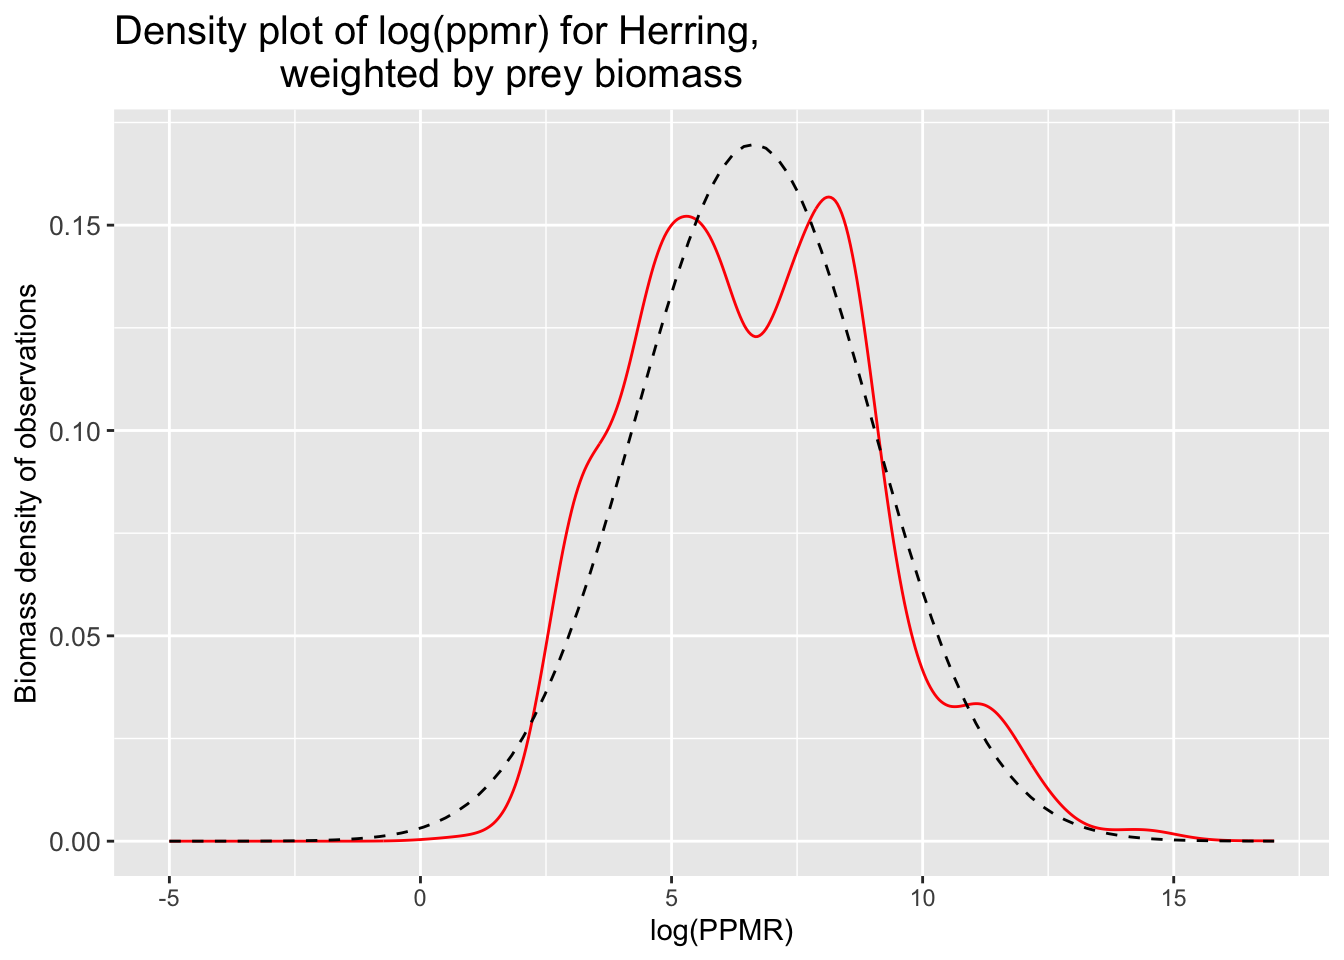
\includegraphics{Trials_files/figure-latex/Prey biomass weighting-1.pdf}

\begin{Shaded}
\begin{Highlighting}[]
\CommentTok{\#stat\_function adds a normal distribution curve (fun=dnorm) with a mean and standard deviation equal to what was calculated earlier for this data set}
\CommentTok{\#xlim sets limits for the x{-}axis so that all the necessary data points can be seen}
\end{Highlighting}
\end{Shaded}

The curve with points weighted by the prey biomass is plotted in blue,
and a normal curve (also weighted by prey biomasss) is plotted over the
top in black.

\hypertarget{weighted-by-number-of-prey-1}{%
\subsection{Weighted by number of
prey}\label{weighted-by-number-of-prey-1}}

\begin{Shaded}
\begin{Highlighting}[]
\NormalTok{no\_herringmean }\OtherTok{=} \FunctionTok{weighted.mean}\NormalTok{(herringDF}\SpecialCharTok{$}\NormalTok{lppmr, }\AttributeTok{w =}\NormalTok{ herringDF}\SpecialCharTok{$}\NormalTok{no.\_prey\_per\_stmch, }\AttributeTok{na.rm =} \ConstantTok{TRUE}\NormalTok{)}
\NormalTok{no\_herringSD }\OtherTok{=} \FunctionTok{sqrt}\NormalTok{(}\FunctionTok{wtd.var}\NormalTok{(herringDF}\SpecialCharTok{$}\NormalTok{lppmr, }\AttributeTok{w =}\NormalTok{ herringDF}\SpecialCharTok{$}\NormalTok{no.\_prey\_per\_stmch, }\AttributeTok{na.rm =} \ConstantTok{TRUE}\NormalTok{))}
\CommentTok{\#the mean and variance are both weighted by the number of prey}

\FunctionTok{paste}\NormalTok{(}\StringTok{"log(ppmr) mean, weighted by number of observations:"}\NormalTok{, no\_herringmean)}
\end{Highlighting}
\end{Shaded}

\begin{verbatim}
## [1] "log(ppmr) mean, weighted by number of observations: 13.5410236346048"
\end{verbatim}

\begin{Shaded}
\begin{Highlighting}[]
\FunctionTok{paste}\NormalTok{(}\StringTok{"Standard deviation of this:"}\NormalTok{, no\_herringSD)}
\end{Highlighting}
\end{Shaded}

\begin{verbatim}
## [1] "Standard deviation of this: 2.63330496940788"
\end{verbatim}

\begin{Shaded}
\begin{Highlighting}[]
\FunctionTok{ggplot}\NormalTok{(}\AttributeTok{data =}\NormalTok{ herringDF, }\FunctionTok{aes}\NormalTok{(}\AttributeTok{x=}\NormalTok{lppmr), }\AttributeTok{group=}\DecValTok{1}\NormalTok{) }\SpecialCharTok{+} 
          \FunctionTok{labs}\NormalTok{(}\AttributeTok{title =} \StringTok{"log(ppmr) against number density for Herring, weighted by no. of prey"}\NormalTok{,}
               \AttributeTok{x=}\StringTok{"log(PPMR)"}\NormalTok{, }\AttributeTok{y=}\StringTok{"No. density of observations"}\NormalTok{) }\SpecialCharTok{+}
          \FunctionTok{geom\_density}\NormalTok{(}\FunctionTok{aes}\NormalTok{(}\AttributeTok{weight =}\NormalTok{ no.\_prey\_per\_stmch), }\AttributeTok{colour=}\StringTok{"red"}\NormalTok{) }\SpecialCharTok{+} 
          \FunctionTok{theme}\NormalTok{(}\AttributeTok{plot.title =} \FunctionTok{element\_text}\NormalTok{(}\AttributeTok{size=}\DecValTok{15}\NormalTok{)) }\SpecialCharTok{+}
          \FunctionTok{stat\_function}\NormalTok{(}\AttributeTok{fun =}\NormalTok{ dnorm, }\AttributeTok{args=} \FunctionTok{with}\NormalTok{(herringDF, }\FunctionTok{c}\NormalTok{(}\AttributeTok{mean =}\NormalTok{ no\_herringmean, }\AttributeTok{sd =}\NormalTok{ no\_herringSD))) }\SpecialCharTok{+}
          \FunctionTok{xlim}\NormalTok{(}\DecValTok{0}\NormalTok{,}\DecValTok{25}\NormalTok{)}
\end{Highlighting}
\end{Shaded}

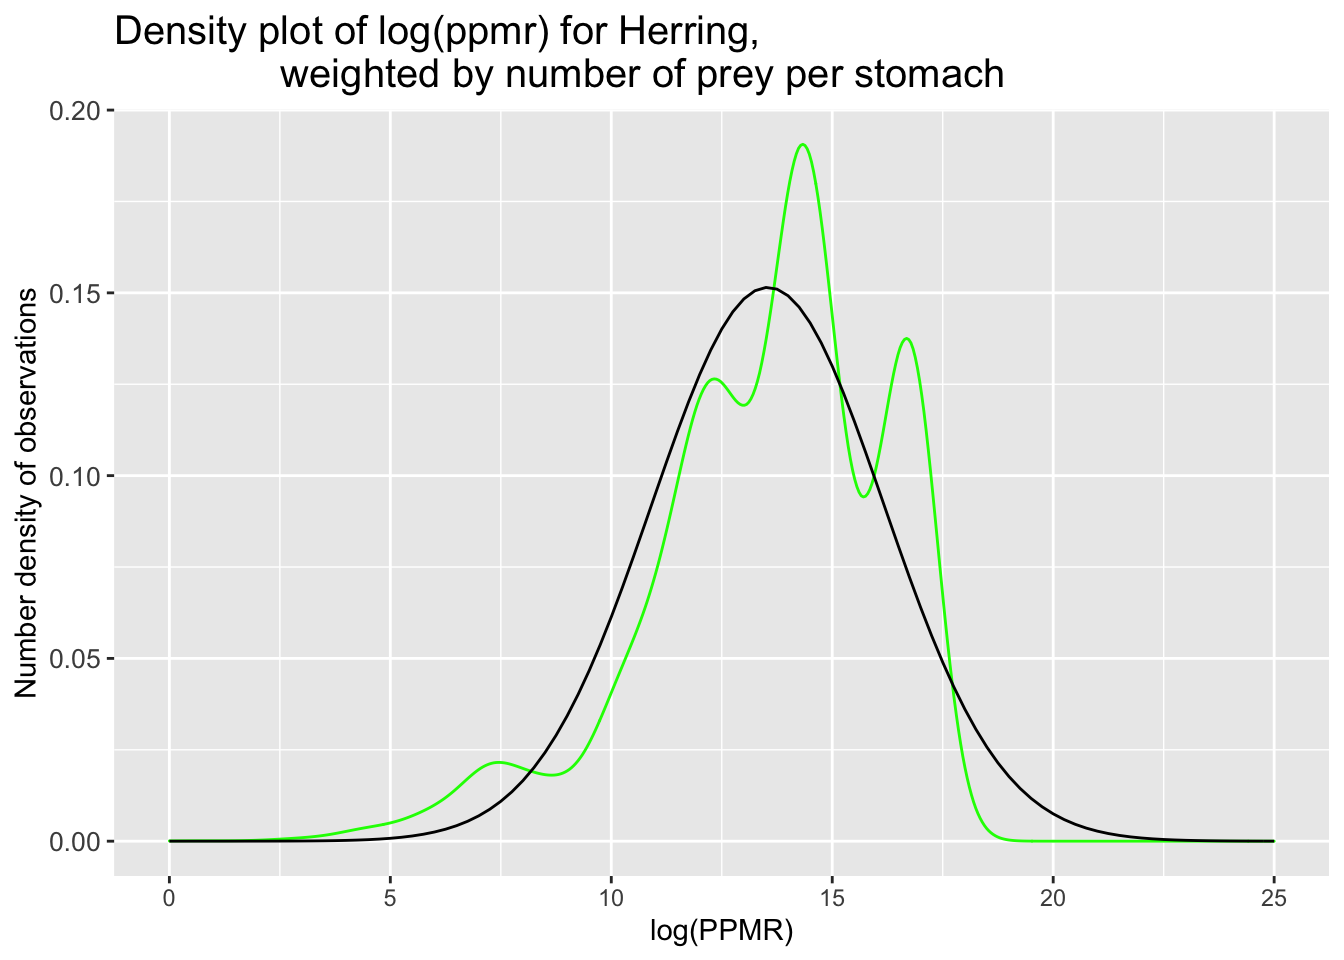
\includegraphics{Trials_files/figure-latex/No of prey weighting-1.pdf}

\begin{Shaded}
\begin{Highlighting}[]
\CommentTok{\#the xlim is different to the graph above because these data points lie over a slightly different log(ppmr) range}
\end{Highlighting}
\end{Shaded}

The curve with points weighted by the number of prey per stomach is
plotted in red, and a normal curve (also weighted by the number of prey
per stomach) is plotted over the top in black.

\hypertarget{combined-graph}{%
\subsection{Combined graph}\label{combined-graph}}

\begin{Shaded}
\begin{Highlighting}[]
\FunctionTok{ggplot}\NormalTok{(}\AttributeTok{data =}\NormalTok{ herringDF, }\FunctionTok{aes}\NormalTok{(}\AttributeTok{x=}\NormalTok{lppmr), }\AttributeTok{group=}\DecValTok{1}\NormalTok{) }\SpecialCharTok{+} 
          \FunctionTok{labs}\NormalTok{(}\AttributeTok{title =} \StringTok{"log(ppmr) against biomass/number density for Herring,}
\StringTok{               with different weightings"}\NormalTok{,}
               \AttributeTok{x=}\StringTok{"log(PPMR)"}\NormalTok{, }\AttributeTok{y=}\StringTok{"Number/biomass density of observations"}\NormalTok{) }\SpecialCharTok{+}
          \FunctionTok{geom\_density}\NormalTok{(}\FunctionTok{aes}\NormalTok{(}\AttributeTok{weight =}\NormalTok{ no.\_prey\_per\_stmch, }\AttributeTok{colour=}\StringTok{"prey biomass"}\NormalTok{)) }\SpecialCharTok{+} 
          \FunctionTok{geom\_density}\NormalTok{(}\FunctionTok{aes}\NormalTok{(}\AttributeTok{weight =}\NormalTok{ prey\_weight\_g, }\AttributeTok{colour=}\StringTok{"number of prey per stomach"}\NormalTok{)) }\SpecialCharTok{+} 
          \FunctionTok{stat\_function}\NormalTok{(}\AttributeTok{fun =}\NormalTok{ dnorm, }\AttributeTok{args=} \FunctionTok{with}\NormalTok{(herringDF, }\FunctionTok{c}\NormalTok{(}\AttributeTok{mean =}\NormalTok{ no\_herringmean, }\AttributeTok{sd =}\NormalTok{ no\_herringSD))) }\SpecialCharTok{+}
          \FunctionTok{stat\_function}\NormalTok{(}\AttributeTok{fun =}\NormalTok{ dnorm, }\AttributeTok{args=} \FunctionTok{with}\NormalTok{(herringDF, }\FunctionTok{c}\NormalTok{(}\AttributeTok{mean =}\NormalTok{ bio\_herringmean, }\AttributeTok{sd =}\NormalTok{ bio\_herringSD))) }\SpecialCharTok{+}
          \FunctionTok{theme}\NormalTok{(}\AttributeTok{plot.title =} \FunctionTok{element\_text}\NormalTok{(}\AttributeTok{size=}\DecValTok{15}\NormalTok{)) }\SpecialCharTok{+}
          \FunctionTok{scale\_color\_manual}\NormalTok{(}\AttributeTok{name=}\StringTok{\textquotesingle{}Weightings\textquotesingle{}}\NormalTok{,}
                     \AttributeTok{values=}\FunctionTok{c}\NormalTok{(}\StringTok{\textquotesingle{}number of prey per stomach\textquotesingle{}}\OtherTok{=}\StringTok{\textquotesingle{}red\textquotesingle{}}\NormalTok{, }\StringTok{\textquotesingle{}prey biomass\textquotesingle{}}\OtherTok{=}\StringTok{\textquotesingle{}blue\textquotesingle{}}\NormalTok{)) }\SpecialCharTok{+}
        \FunctionTok{xlim}\NormalTok{(}\SpecialCharTok{{-}}\DecValTok{5}\NormalTok{,}\DecValTok{25}\NormalTok{) }
\end{Highlighting}
\end{Shaded}

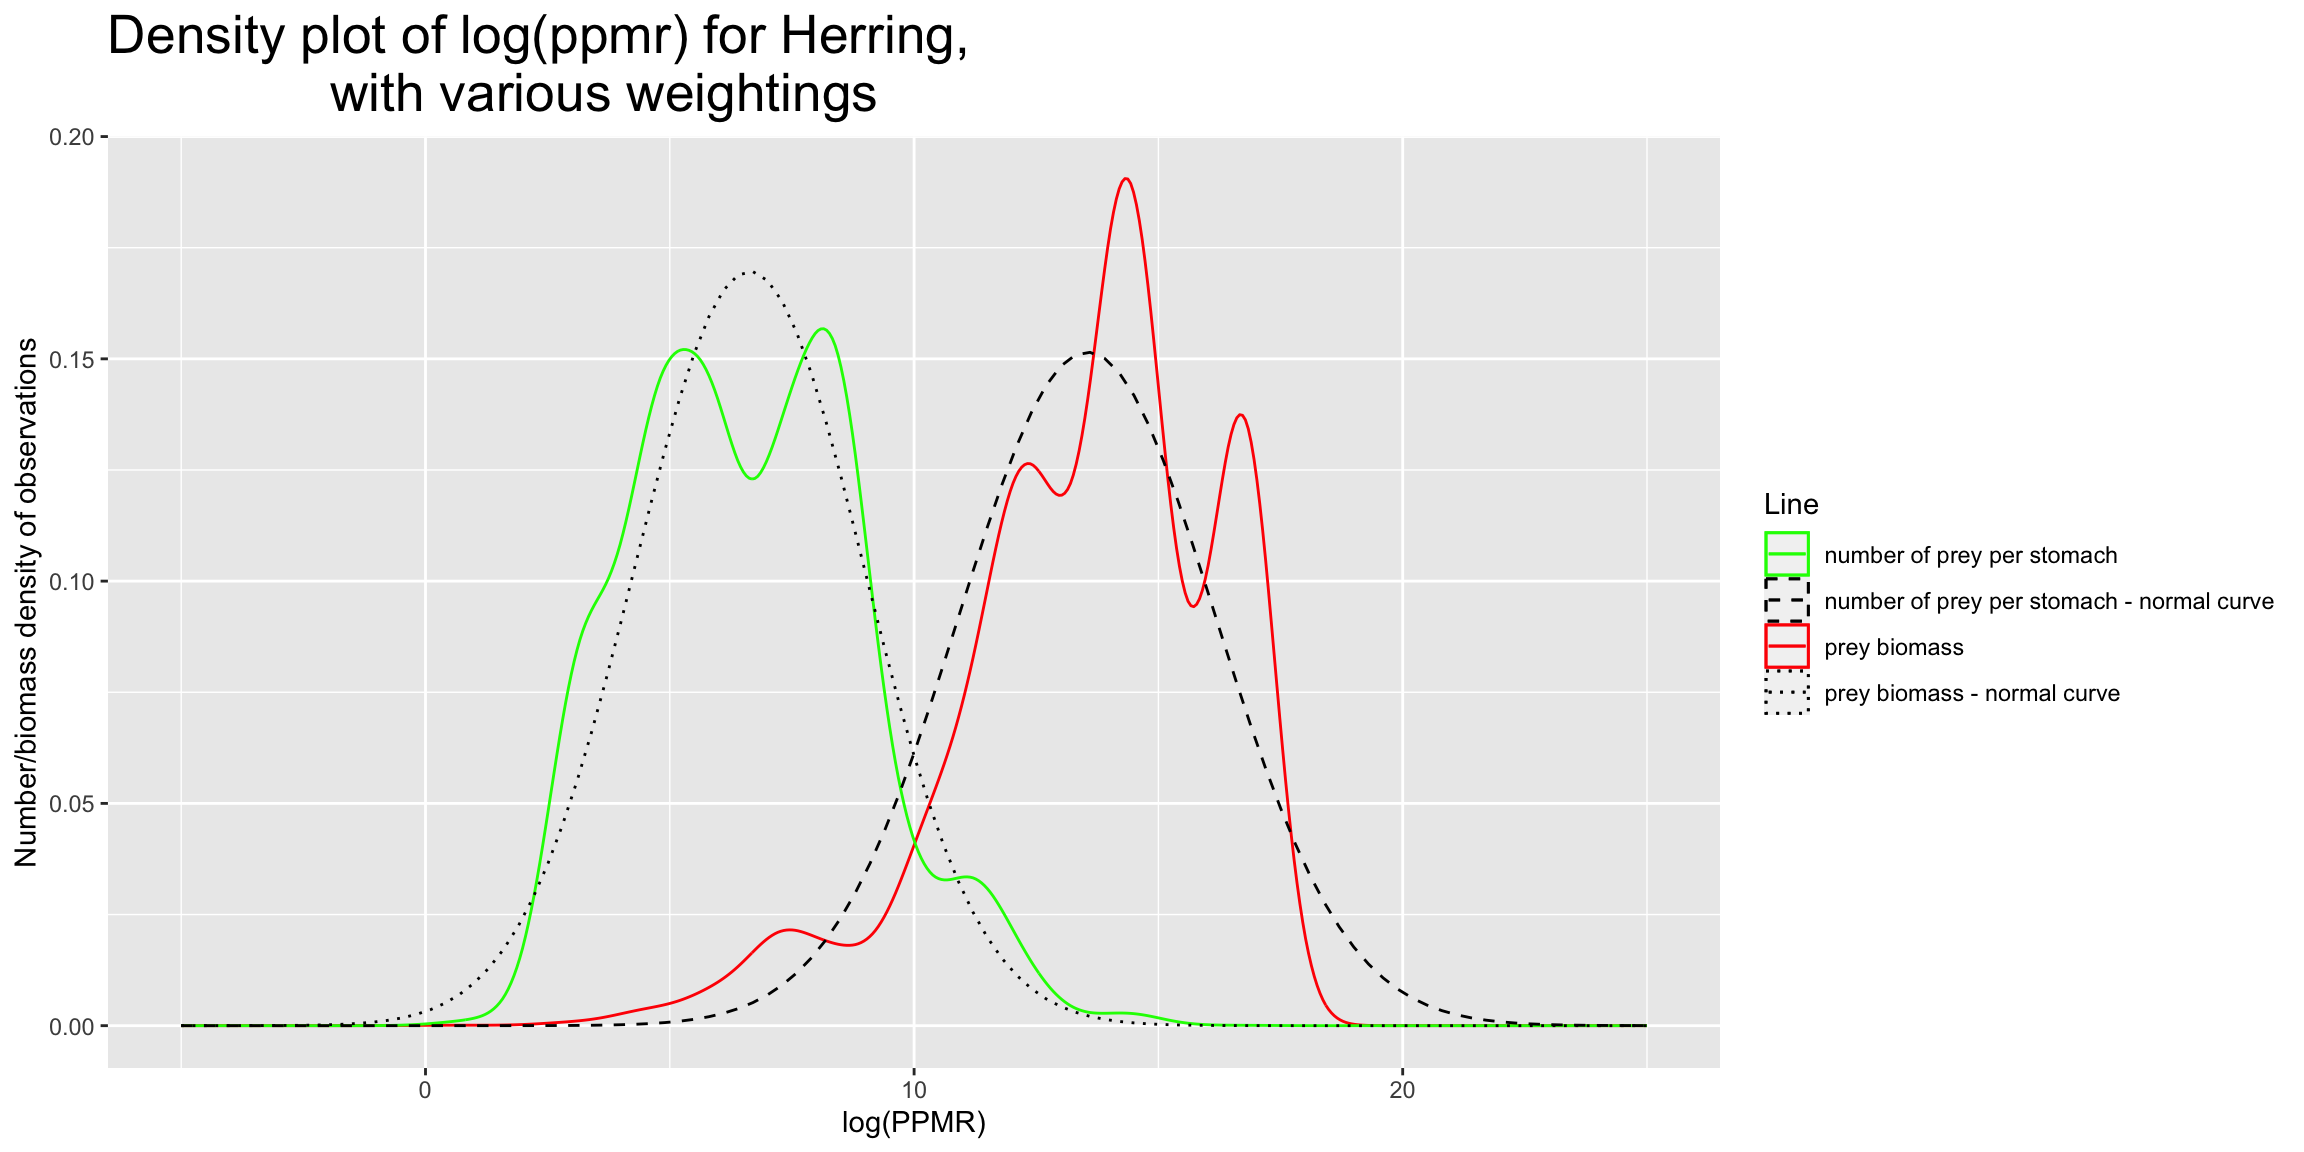
\includegraphics{Trials_files/figure-latex/Herring combined graph-1.pdf}

\begin{Shaded}
\begin{Highlighting}[]
\CommentTok{\#scale\_color\_manual manually adds a key to the graph to describe what the differently coloured lines represent}
\CommentTok{\#each curve is given a name using \textquotesingle{}aes(colour="")\textquotesingle{}, and these are then given a specific colour using \textquotesingle{}values=\textquotesingle{}}
\end{Highlighting}
\end{Shaded}

This is a graph with both the the distribution of Herring log(PPMR) as
weighted by prey biomass and number of prey plotted over each other
(along with appropriately weighted normal distribution curves plotted
over the top of each).

Prey biomass weighted mean: 6.629177 No.~of prey weighted mean: 13.54102

Prey biomass standard deviation: 2.3508789268221 No.~of prey standard
deviation: 2.63330496940788

The mean is shifted by 6.911843.

The mathematics of shifted means for this difference in weighting is:

\[
  \text{weighted mean}_{\text{expected prey biomass}} = \text{weighted mean}_{\text{no. of prey }} - (\text{standard deviation}_{\text{no. of prey }})^2
\]

Hence, the expected result is:

\[
  \text{weighted mean}_{\text{actual prey biomass}} = 13.54102 - (2.63330496940788)^2 = 6.60672493809
\] There is a difference in expected and actual prey biomass weighted
mean of 0.30511806191. This is a fairly insignificant value, which
suggests the shifting mean equations are relatively accurate for this
data set with these weightings.

Therefore, we can continue with the assumption that there is a
difference in the mean of log(ppmr) of the square of the standard
deviation when we weight by number of prey per stomach and prey biomass.

\hypertarget{introducing-a-mixed-effects-model}{%
\section{Introducing a mixed effects
model}\label{introducing-a-mixed-effects-model}}

\hypertarget{building-up-the-model}{%
\subsection{Building up the model}\label{building-up-the-model}}

\hypertarget{basic-linear-model}{%
\subsubsection{Basic Linear model}\label{basic-linear-model}}

With \$\log(\text{prey_weight}) = m \times \log(\text{pred_species}) + c

\begin{Shaded}
\begin{Highlighting}[]
\NormalTok{renamed\_df }\SpecialCharTok{\%\textgreater{}\%} 
    \FunctionTok{ggplot}\NormalTok{(}\FunctionTok{aes}\NormalTok{(}\AttributeTok{x=}\NormalTok{lprey\_weight, }\AttributeTok{y=}\NormalTok{lppmr, }\AttributeTok{group=}\NormalTok{pred\_species, }\AttributeTok{color=}\NormalTok{pred\_species)) }\SpecialCharTok{+} 
    \FunctionTok{geom\_line}\NormalTok{(}\AttributeTok{size=}\DecValTok{1}\NormalTok{) }\SpecialCharTok{+} \FunctionTok{theme\_classic}\NormalTok{()}
\end{Highlighting}
\end{Shaded}

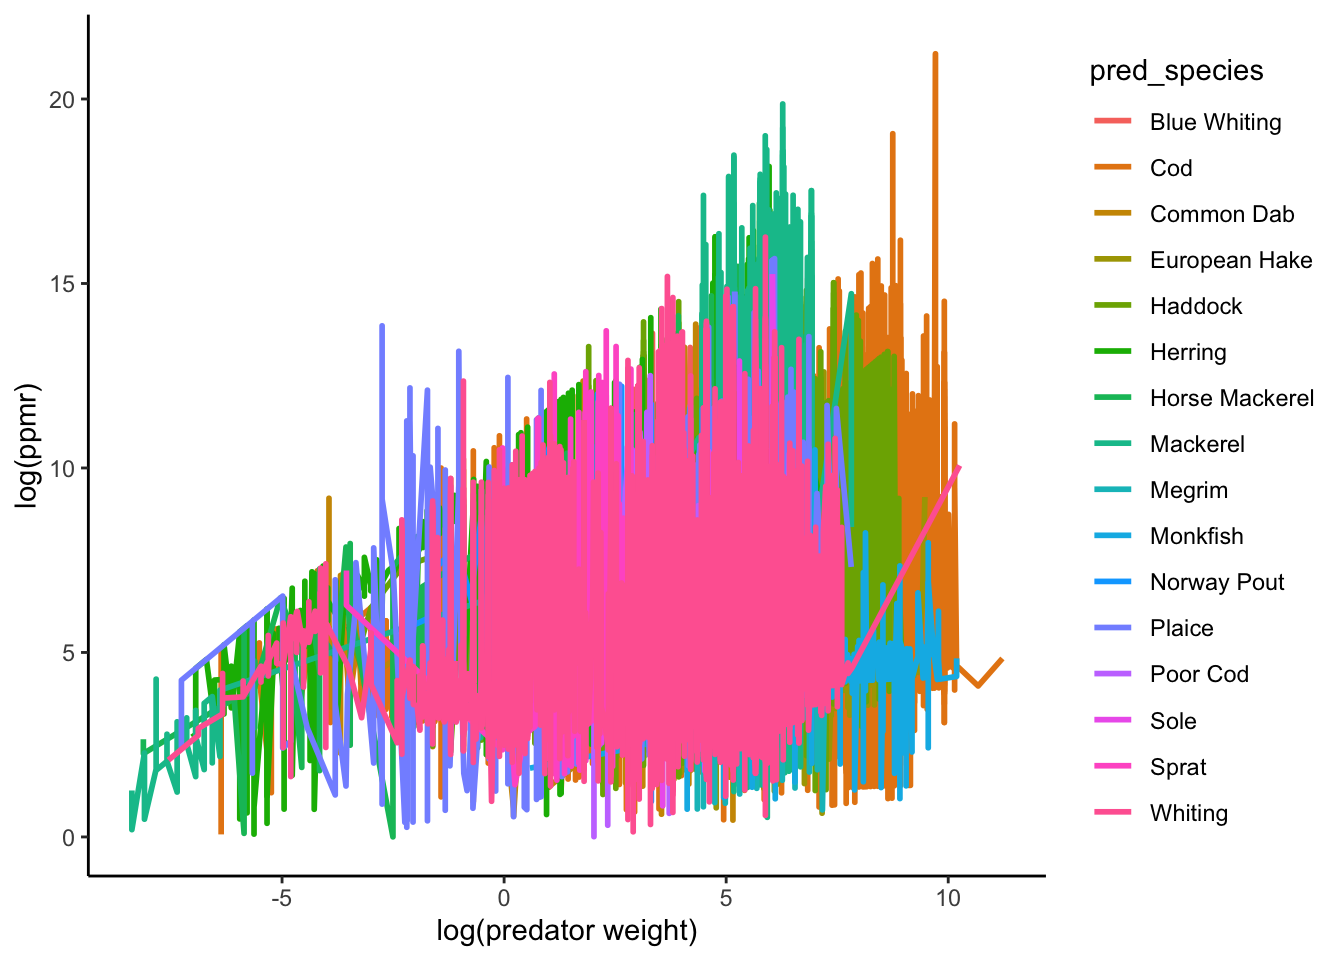
\includegraphics{Trials_files/figure-latex/linear model-1.pdf}

\hypertarget{null}{%
\subsubsection{Null}\label{null}}

Fixed effects: no fixed effects

Renamed effects: pred\_species

\begin{Shaded}
\begin{Highlighting}[]
\NormalTok{null }\OtherTok{\textless{}{-}} \FunctionTok{lmer}\NormalTok{(lppmr }\SpecialCharTok{\textasciitilde{}}\NormalTok{ (}\DecValTok{1}\SpecialCharTok{|}\NormalTok{pred\_species), }\AttributeTok{data =}\NormalTok{ renamed\_df, }\AttributeTok{REML=}\ConstantTok{FALSE}\NormalTok{)}
\CommentTok{\#the \textquotesingle{}null\textquotesingle{} model has no predictors (i.e. no linear effects)}
\CommentTok{\#REML=FALSE means the model is made using \textquotesingle{}maximum likelihood\textquotesingle{} (rather than Restricted Maximum Likelihood), which allows us to compare different models}

\NormalTok{renamed\_df }\SpecialCharTok{\%\textgreater{}\%} 
    \FunctionTok{mutate}\NormalTok{(}\AttributeTok{lppmr =} \FunctionTok{fitted}\NormalTok{(null)) }\SpecialCharTok{\%\textgreater{}\%} 
    \FunctionTok{ggplot}\NormalTok{(}\FunctionTok{aes}\NormalTok{(}\AttributeTok{x=}\NormalTok{lprey\_weight, }\AttributeTok{y=}\NormalTok{lppmr, }\AttributeTok{group=}\NormalTok{pred\_species, }\AttributeTok{color=}\NormalTok{pred\_species)) }\SpecialCharTok{+}
    \FunctionTok{theme\_classic}\NormalTok{() }\SpecialCharTok{+}
    \FunctionTok{geom\_line}\NormalTok{(}\AttributeTok{size=}\DecValTok{1}\NormalTok{) }
\end{Highlighting}
\end{Shaded}

\includegraphics{Trials_files/figure-latex/null model-1.pdf}

Mathematical representation: \[
    \log(\text{ppmr})_{ij} = \beta_{0} + S_{0[j]} + \epsilon_{ij}
\]

This model has the following variables:

\begin{itemize}
  * $i$ is the group
  * $j$ is the item
  * $\beta_{0}$ is the intercept term (grand mean)
  * $S_{0[j]}$ is the effect of the random term (pred_species)
  * $\epsilon_{ij}$ is the error term.
\end{itemize}

\hypertarget{first-trial}{%
\subsubsection{First trial}\label{first-trial}}

Fixed effects: lprey\_weight

Renamed effects: pred\_species

\begin{Shaded}
\begin{Highlighting}[]
\NormalTok{one }\OtherTok{\textless{}{-}} \FunctionTok{lmer}\NormalTok{(lppmr }\SpecialCharTok{\textasciitilde{}}\NormalTok{ lprey\_weight }\SpecialCharTok{+}\NormalTok{ (}\DecValTok{1}\SpecialCharTok{|}\NormalTok{pred\_species), }\AttributeTok{data =}\NormalTok{ renamed\_df, }\AttributeTok{REML=}\ConstantTok{FALSE}\NormalTok{)}
\CommentTok{\#same slope for every effect (but varying intercept)}

\NormalTok{renamed\_df }\SpecialCharTok{\%\textgreater{}\%} 
    \FunctionTok{mutate}\NormalTok{(}\AttributeTok{lppmr=} \FunctionTok{fitted}\NormalTok{(one)) }\SpecialCharTok{\%\textgreater{}\%} 
    \FunctionTok{ggplot}\NormalTok{(}\FunctionTok{aes}\NormalTok{(}\AttributeTok{x=}\NormalTok{lprey\_weight, }\AttributeTok{y=}\NormalTok{lppmr, }\AttributeTok{group=}\NormalTok{pred\_species, }\AttributeTok{color=}\NormalTok{pred\_species)) }\SpecialCharTok{+} 
    \FunctionTok{theme\_classic}\NormalTok{() }\SpecialCharTok{+}
    \FunctionTok{geom\_line}\NormalTok{(}\AttributeTok{size=}\DecValTok{1}\NormalTok{) }
\end{Highlighting}
\end{Shaded}

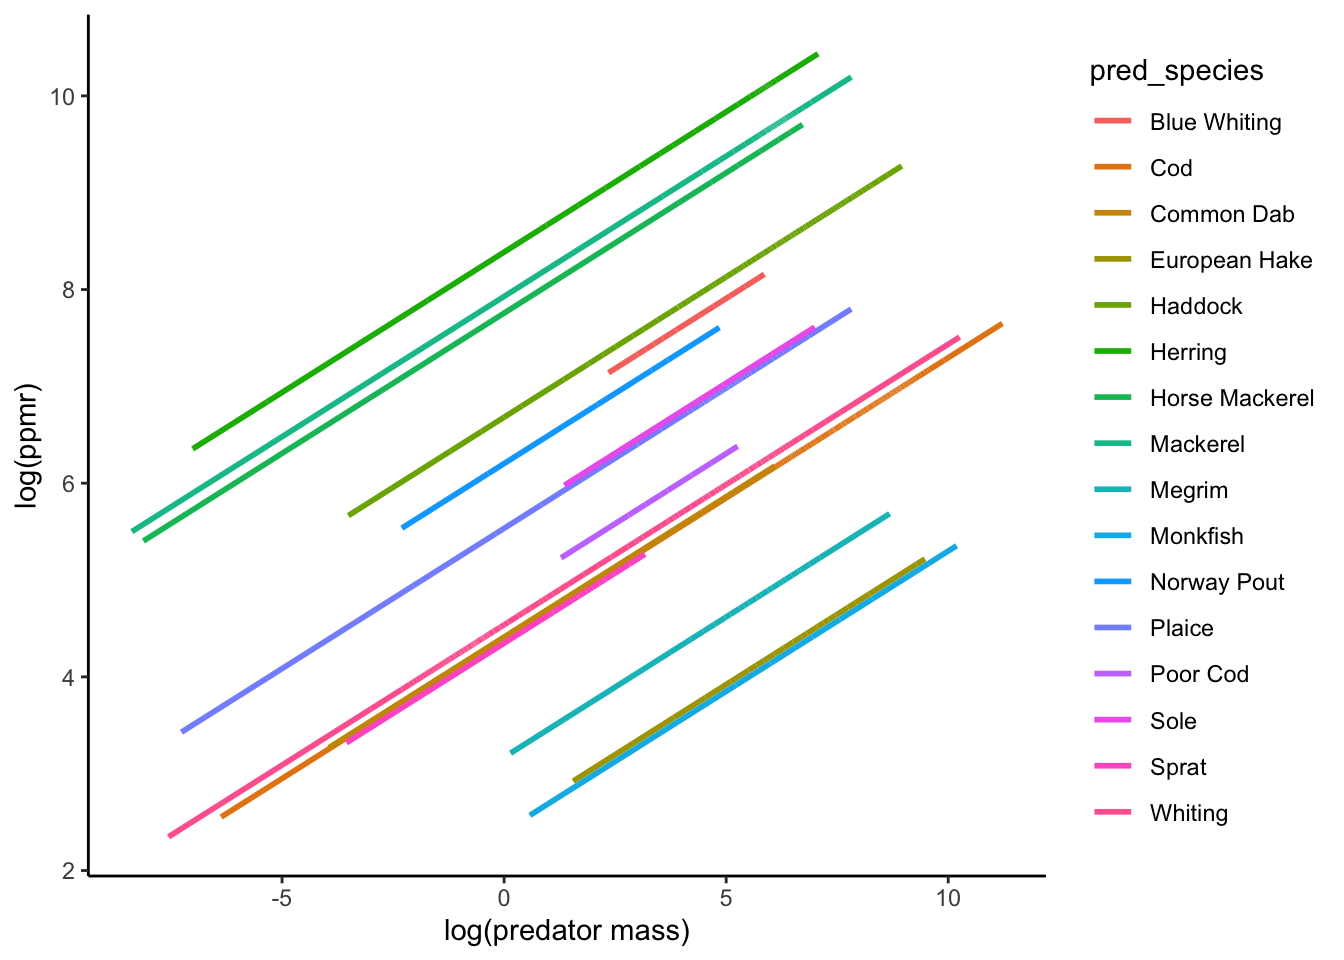
\includegraphics{Trials_files/figure-latex/first-1.pdf}

\hypertarget{second-trial}{%
\subsubsection{Second trial}\label{second-trial}}

Fixed effects: lprey\_weight

Renamed effects: pred\_species (random slope and fixed intercept; varies
w.r.t lprey\_weight)

\begin{Shaded}
\begin{Highlighting}[]
\NormalTok{two }\OtherTok{\textless{}{-}} \FunctionTok{lmer}\NormalTok{(lppmr }\SpecialCharTok{\textasciitilde{}}\NormalTok{ lprey\_weight }\SpecialCharTok{+}\NormalTok{ (}\DecValTok{0}\SpecialCharTok{+}\NormalTok{lprey\_weight}\SpecialCharTok{|}\NormalTok{pred\_species), }\AttributeTok{data =}\NormalTok{ renamed\_df, }\AttributeTok{REML=}\ConstantTok{FALSE}\NormalTok{)}
\CommentTok{\#Random intercept and random slope (independent)}

\NormalTok{renamed\_df }\SpecialCharTok{\%\textgreater{}\%} 
    \FunctionTok{mutate}\NormalTok{(}\AttributeTok{lppmr =} \FunctionTok{fitted}\NormalTok{(two)) }\SpecialCharTok{\%\textgreater{}\%} 
    \FunctionTok{ggplot}\NormalTok{(}\FunctionTok{aes}\NormalTok{(}\AttributeTok{x=}\NormalTok{lprey\_weight, }\AttributeTok{y=}\NormalTok{lppmr, }\AttributeTok{group=}\NormalTok{pred\_species, }\AttributeTok{color=}\NormalTok{pred\_species)) }\SpecialCharTok{+} 
    \FunctionTok{theme\_classic}\NormalTok{() }\SpecialCharTok{+}
    \FunctionTok{geom\_line}\NormalTok{(}\AttributeTok{size=}\DecValTok{1}\NormalTok{) }
\end{Highlighting}
\end{Shaded}

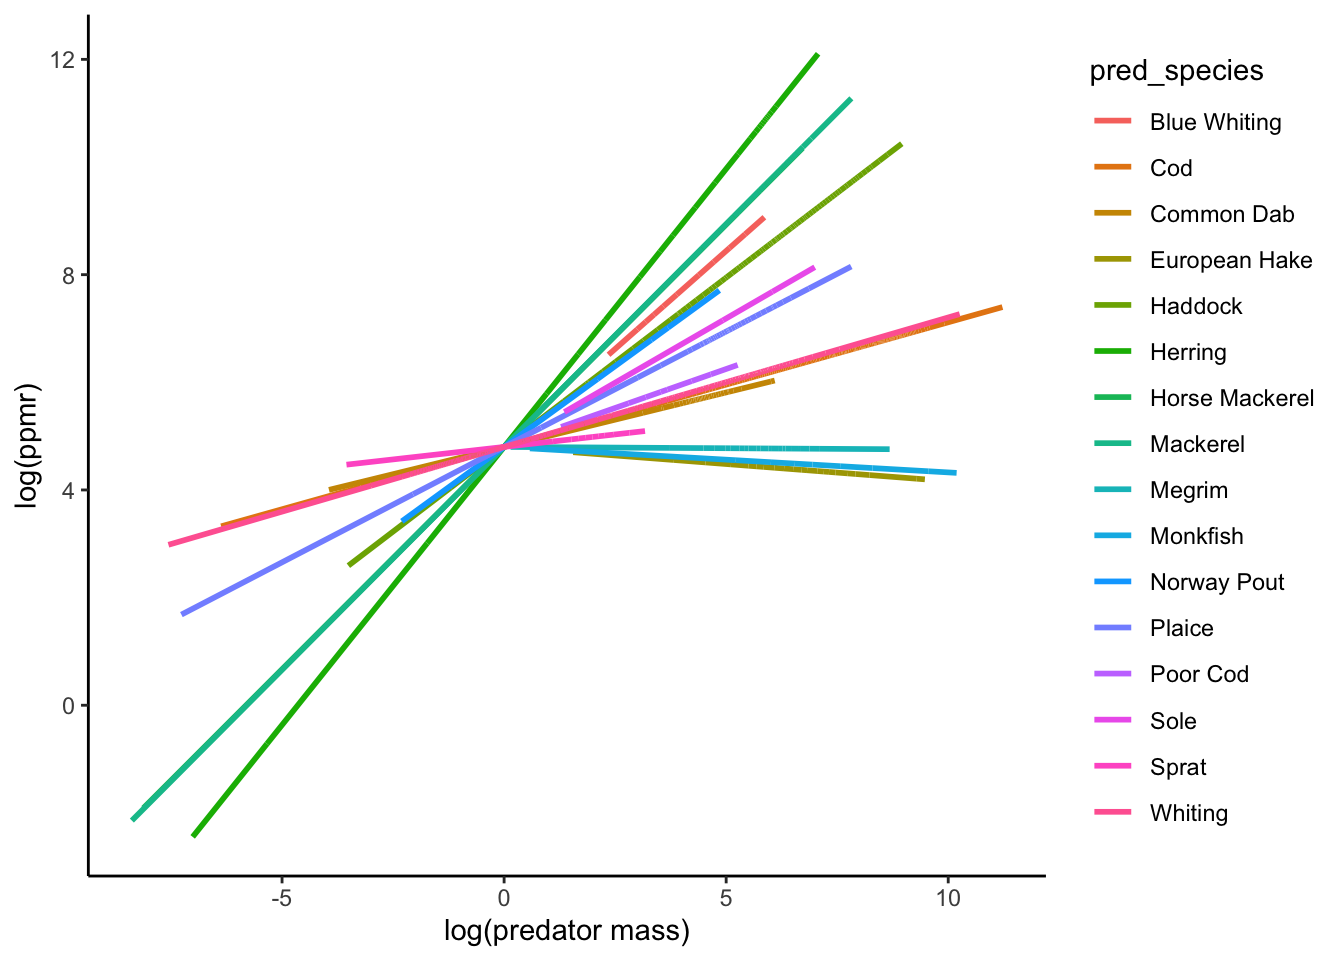
\includegraphics{Trials_files/figure-latex/second-1.pdf}

\hypertarget{third-trial}{%
\subsubsection{Third trial}\label{third-trial}}

Fixed effects: lprey\_weight

Renamed effects: pred\_species (random slope and random intercept;
varies w.r.t lprey\_weight)

\begin{Shaded}
\begin{Highlighting}[]
\NormalTok{three }\OtherTok{\textless{}{-}} \FunctionTok{lmer}\NormalTok{(lppmr }\SpecialCharTok{\textasciitilde{}}\NormalTok{ lprey\_weight }\SpecialCharTok{+}\NormalTok{ (}\DecValTok{1}\SpecialCharTok{+}\NormalTok{lprey\_weight}\SpecialCharTok{|}\NormalTok{pred\_species), }\AttributeTok{data =}\NormalTok{ renamed\_df, }\AttributeTok{REML=}\ConstantTok{FALSE}\NormalTok{)}
\CommentTok{\#Random intercept and random slope (correlated)}

\NormalTok{renamed\_df }\SpecialCharTok{\%\textgreater{}\%} 
    \FunctionTok{mutate}\NormalTok{(}\AttributeTok{lppmr =} \FunctionTok{fitted}\NormalTok{(three)) }\SpecialCharTok{\%\textgreater{}\%} 
    \FunctionTok{ggplot}\NormalTok{(}\FunctionTok{aes}\NormalTok{(}\AttributeTok{x=}\NormalTok{lprey\_weight, }\AttributeTok{y=}\NormalTok{lppmr, }\AttributeTok{group=}\NormalTok{pred\_species, }\AttributeTok{color=}\NormalTok{pred\_species)) }\SpecialCharTok{+} 
    \FunctionTok{theme\_classic}\NormalTok{() }\SpecialCharTok{+}
    \FunctionTok{geom\_line}\NormalTok{(}\AttributeTok{size=}\DecValTok{1}\NormalTok{) }
\end{Highlighting}
\end{Shaded}

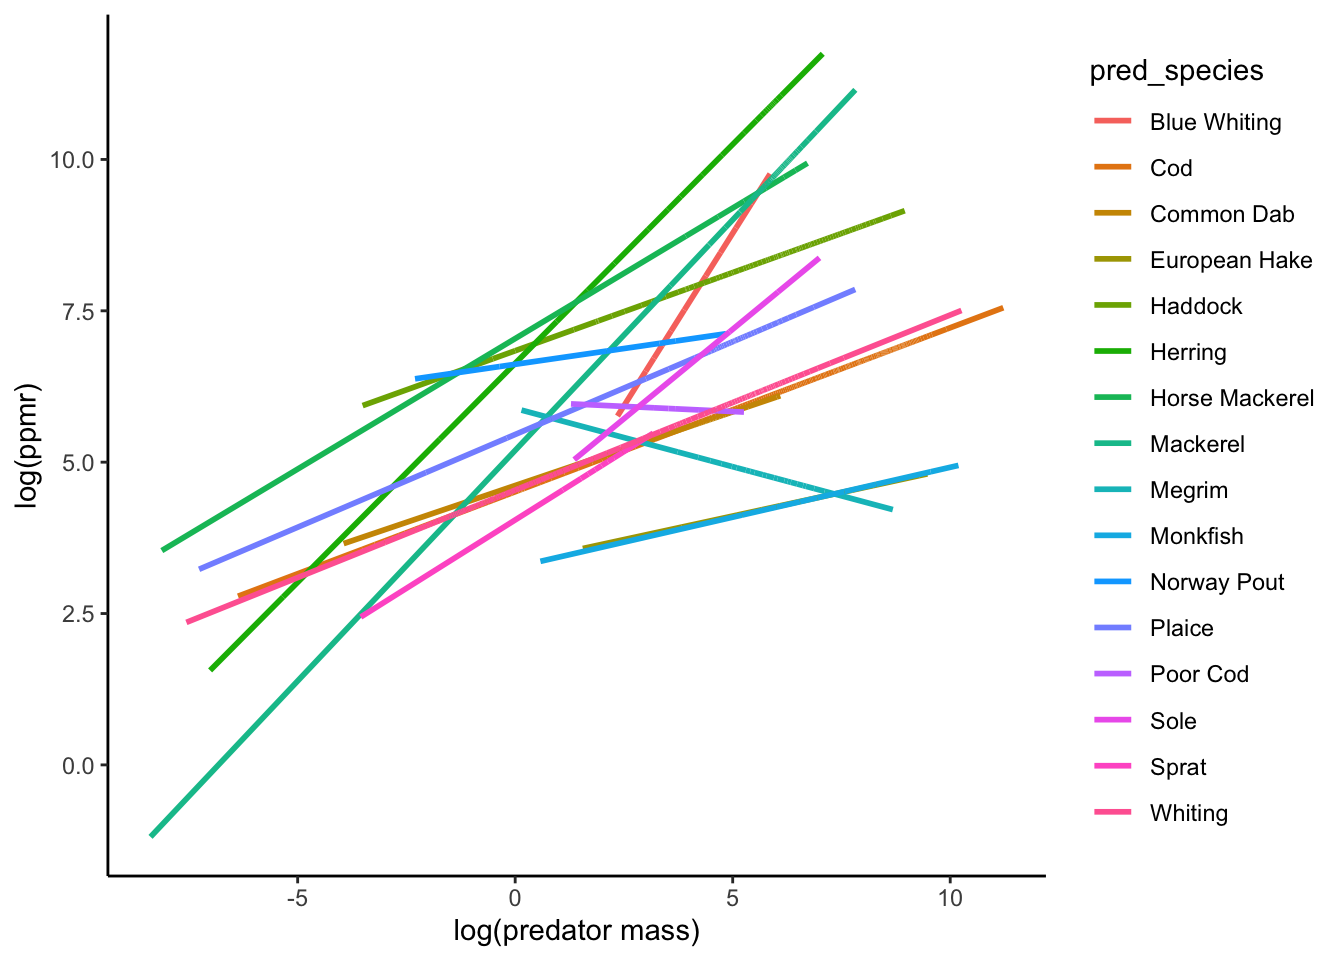
\includegraphics{Trials_files/figure-latex/third-1.pdf}

\hypertarget{comparing-the-model}{%
\subsubsection{Comparing the model}\label{comparing-the-model}}

\begin{Shaded}
\begin{Highlighting}[]
\FunctionTok{anova}\NormalTok{(null,one,two,three)}
\end{Highlighting}
\end{Shaded}

\begin{verbatim}
## Data: renamed_df
## Models:
## null: lppmr ~ (1 | pred_species)
## one: lppmr ~ lprey_weight + (1 | pred_species)
## two: lppmr ~ lprey_weight + (0 + lprey_weight | pred_species)
## three: lppmr ~ lprey_weight + (1 + lprey_weight | pred_species)
##       npar     AIC     BIC  logLik deviance  Chisq Df Pr(>Chisq)    
## null     3 1188058 1188090 -594026  1188052                         
## one      4 1084789 1084831 -542391  1084781 103271  1  < 2.2e-16 ***
## two      4 1047701 1047743 -523847  1047693  37088  0               
## three    6 1024125 1024188 -512057  1024113  23580  2  < 2.2e-16 ***
## ---
## Signif. codes:  0 '***' 0.001 '**' 0.01 '*' 0.05 '.' 0.1 ' ' 1
\end{verbatim}

\begin{Shaded}
\begin{Highlighting}[]
\CommentTok{\#comparing the four models}

\CommentTok{\#(1+lprey\_weight|pred\_species)}
\CommentTok{\#(1+pred\_species|haul\_id\_short) {-}{-}\textgreater{} doesn\textquotesingle{}t compile?}
\CommentTok{\#couldn\textquotesingle{}t introduce (1+pred\_species|haul\_id\_short) or (1+lprey\_weight|haul\_id\_short)}
\end{Highlighting}
\end{Shaded}

\hypertarget{trialing-different-models}{%
\subsection{Trialing different models}\label{trialing-different-models}}

Here, all the random effects are modelled with a randomly distributed
slope and intercept.

\hypertarget{trial-a}{%
\subsubsection{Trial a}\label{trial-a}}

Fixed effects: lprey\_weight

Renamed effects: haul\_id\_short

\begin{Shaded}
\begin{Highlighting}[]
\NormalTok{a }\OtherTok{\textless{}{-}} \FunctionTok{lmer}\NormalTok{(lppmr }\SpecialCharTok{\textasciitilde{}}\NormalTok{ lprey\_weight }\SpecialCharTok{+}\NormalTok{ (}\DecValTok{1}\SpecialCharTok{|}\NormalTok{haul\_id\_short), }\AttributeTok{data =}\NormalTok{ renamed\_df, }\AttributeTok{REML=}\ConstantTok{FALSE}\NormalTok{)}
\NormalTok{a}
\end{Highlighting}
\end{Shaded}

\begin{verbatim}
## Linear mixed model fit by maximum likelihood  ['lmerMod']
## Formula: lppmr ~ lprey_weight + (1 | haul_id_short)
##    Data: renamed_df
##       AIC       BIC    logLik  deviance  df.resid 
##  837098.1  837140.1 -418545.1  837090.1    267427 
## Random effects:
##  Groups        Name        Std.Dev.
##  haul_id_short (Intercept) 1.937   
##  Residual                  1.156   
## Number of obs: 267431, groups:  haul_id_short, 110
## Fixed Effects:
##  (Intercept)  lprey_weight  
##       5.1547       -0.7336
\end{verbatim}

\begin{Shaded}
\begin{Highlighting}[]
\FunctionTok{hist}\NormalTok{(}\FunctionTok{resid}\NormalTok{(a), }\AttributeTok{border=}\StringTok{\textquotesingle{}red\textquotesingle{}}\NormalTok{, }\AttributeTok{col=}\StringTok{"transparent"}\NormalTok{, }\AttributeTok{main =} \FunctionTok{paste}\NormalTok{(}\StringTok{"Histogram of residuals"}\NormalTok{ ))}
\end{Highlighting}
\end{Shaded}

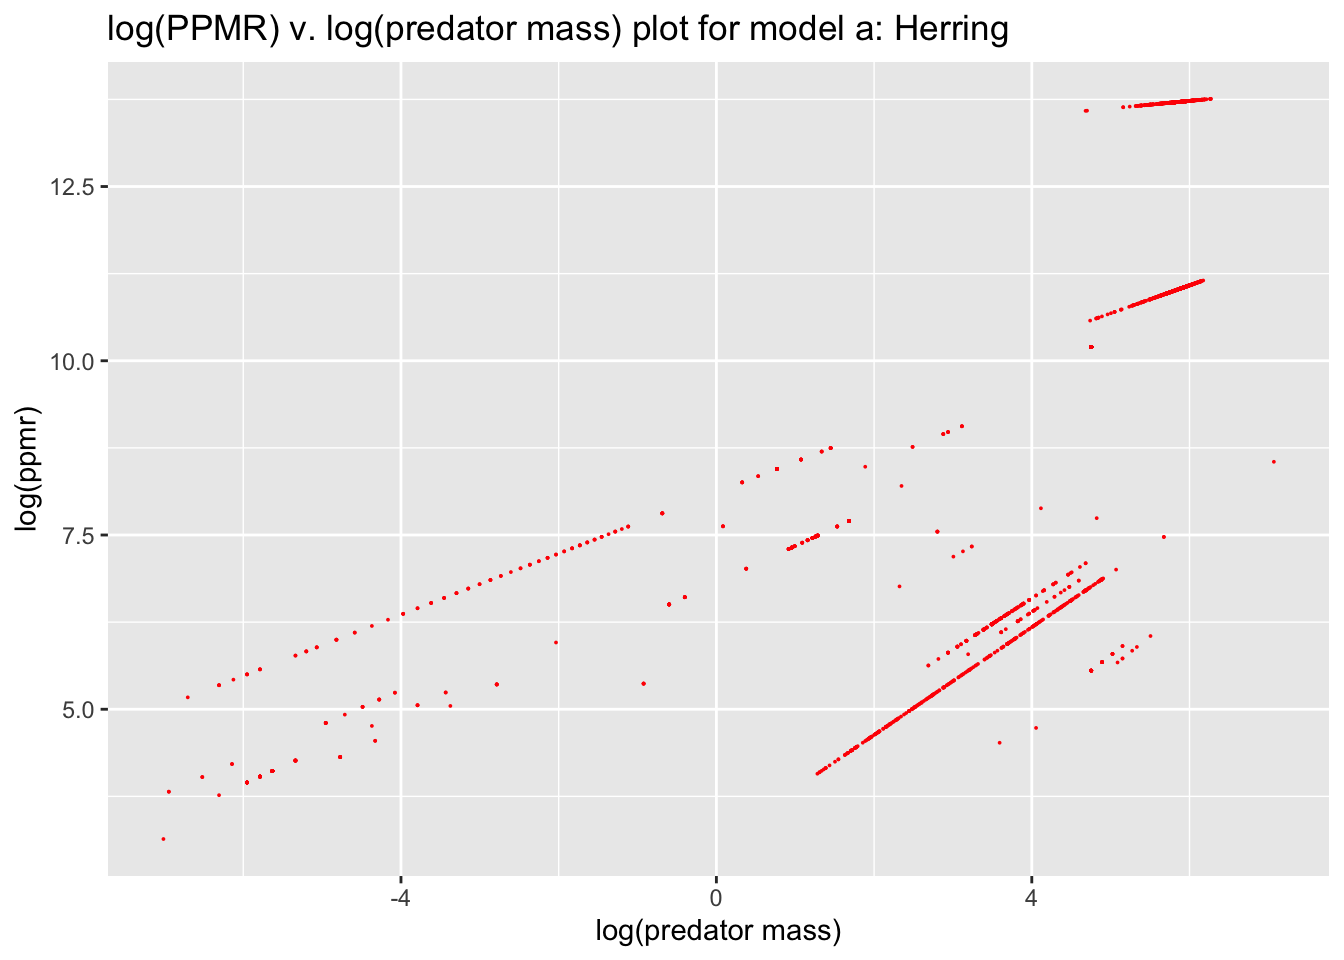
\includegraphics{Trials_files/figure-latex/trial a-1.pdf}

\begin{Shaded}
\begin{Highlighting}[]
\CommentTok{\#Creates a histogram of the distribution of the residuals}
\FunctionTok{print}\NormalTok{(}\FunctionTok{VarCorr}\NormalTok{(a),}\AttributeTok{comp=}\StringTok{"Variance"}\NormalTok{)}
\end{Highlighting}
\end{Shaded}

\begin{verbatim}
##  Groups        Name        Variance
##  haul_id_short (Intercept) 3.7532  
##  Residual                  1.3358
\end{verbatim}

\begin{Shaded}
\begin{Highlighting}[]
\CommentTok{\#Only prints the variance estimates for the random effects}
\FunctionTok{paste}\NormalTok{(}\StringTok{"AIC:"}\NormalTok{, }\FunctionTok{AIC}\NormalTok{(a))}
\end{Highlighting}
\end{Shaded}

\begin{verbatim}
## [1] "AIC: 837098.118608064"
\end{verbatim}

\begin{Shaded}
\begin{Highlighting}[]
\CommentTok{\#Prints the AIC value for this model}
\end{Highlighting}
\end{Shaded}

\hypertarget{trial-b}{%
\subsubsection{Trial b}\label{trial-b}}

Fixed effects: lprey\_weight

Renamed effects: haul\_id\_short, year

\begin{Shaded}
\begin{Highlighting}[]
\NormalTok{b }\OtherTok{\textless{}{-}} \FunctionTok{lmer}\NormalTok{(lppmr }\SpecialCharTok{\textasciitilde{}}\NormalTok{ lprey\_weight }\SpecialCharTok{+}\NormalTok{ (}\DecValTok{1}\SpecialCharTok{|}\NormalTok{haul\_id\_short) }\SpecialCharTok{+}\NormalTok{ (}\DecValTok{1}\SpecialCharTok{|}\NormalTok{year), }\AttributeTok{data =}\NormalTok{ renamed\_df, }\AttributeTok{REML=}\ConstantTok{FALSE}\NormalTok{)}
\NormalTok{b}
\end{Highlighting}
\end{Shaded}

\begin{verbatim}
## Linear mixed model fit by maximum likelihood  ['lmerMod']
## Formula: lppmr ~ lprey_weight + (1 | haul_id_short) + (1 | year)
##    Data: renamed_df
##       AIC       BIC    logLik  deviance  df.resid 
##  826114.8  826167.2 -413052.4  826104.8    267263 
## Random effects:
##  Groups        Name        Std.Dev.
##  haul_id_short (Intercept) 1.991   
##  year          (Intercept) 1.329   
##  Residual                  1.132   
## Number of obs: 267268, groups:  haul_id_short, 110; year, 100
## Fixed Effects:
##  (Intercept)  lprey_weight  
##       5.1602       -0.7405
\end{verbatim}

\begin{Shaded}
\begin{Highlighting}[]
\FunctionTok{hist}\NormalTok{(}\FunctionTok{resid}\NormalTok{(b), }\AttributeTok{border=}\StringTok{\textquotesingle{}red\textquotesingle{}}\NormalTok{, }\AttributeTok{col=}\StringTok{"transparent"}\NormalTok{, }\AttributeTok{main =} \FunctionTok{paste}\NormalTok{(}\StringTok{"Histogram of residuals"}\NormalTok{ ))}
\end{Highlighting}
\end{Shaded}

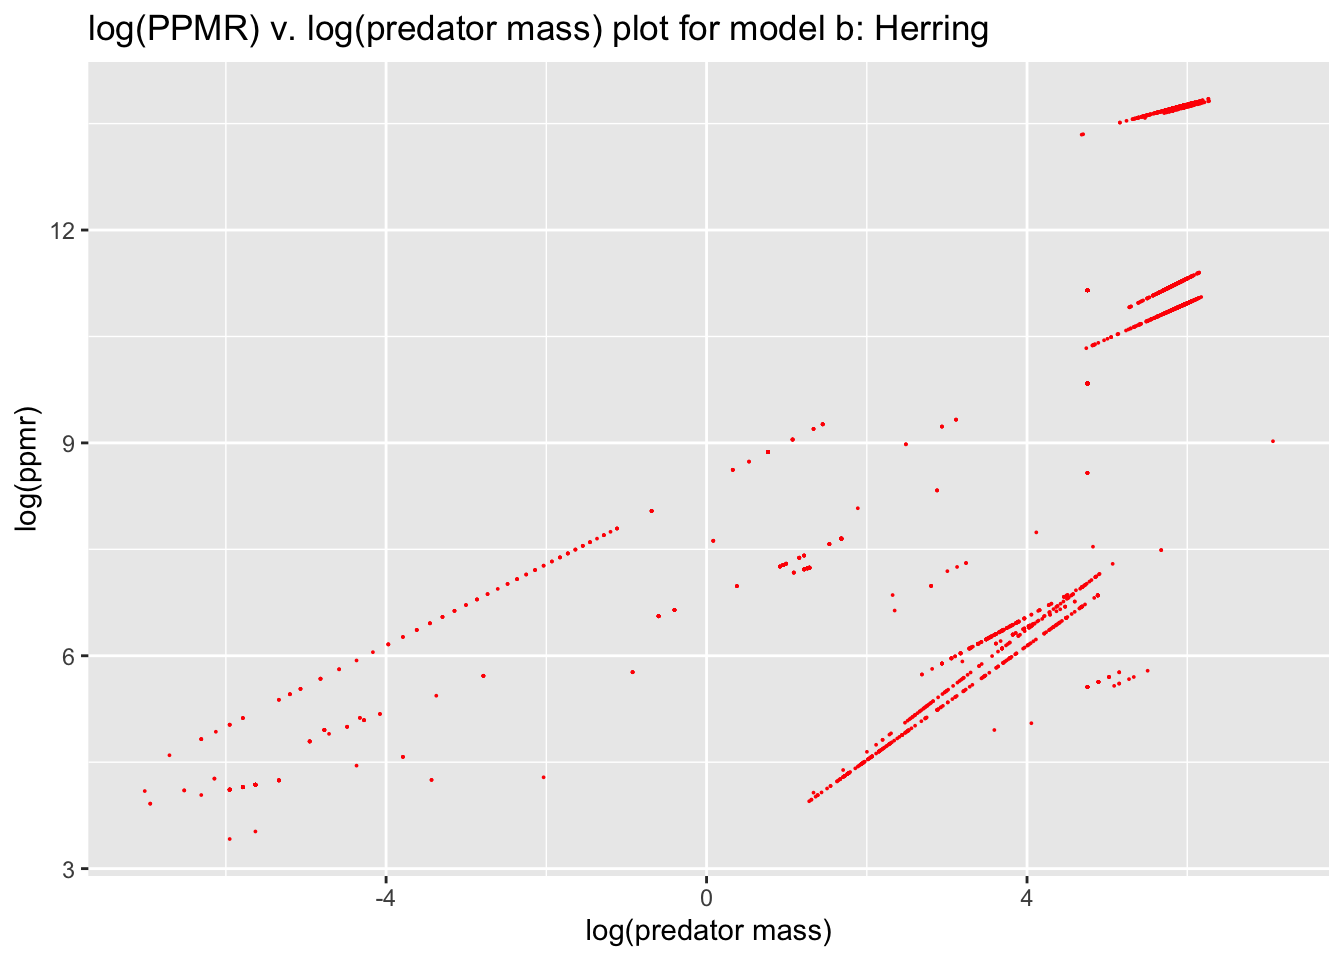
\includegraphics{Trials_files/figure-latex/trial b-1.pdf}

\begin{Shaded}
\begin{Highlighting}[]
\FunctionTok{print}\NormalTok{(}\FunctionTok{VarCorr}\NormalTok{(b),}\AttributeTok{comp=}\StringTok{"Variance"}\NormalTok{)}
\end{Highlighting}
\end{Shaded}

\begin{verbatim}
##  Groups        Name        Variance
##  haul_id_short (Intercept) 3.9630  
##  year          (Intercept) 1.7655  
##  Residual                  1.2824
\end{verbatim}

\begin{Shaded}
\begin{Highlighting}[]
\FunctionTok{paste}\NormalTok{(}\StringTok{"AIC:"}\NormalTok{, }\FunctionTok{AIC}\NormalTok{(b))}
\end{Highlighting}
\end{Shaded}

\begin{verbatim}
## [1] "AIC: 826114.763528339"
\end{verbatim}

\hypertarget{trial-c}{%
\subsubsection{Trial c}\label{trial-c}}

Fixed effects: lprey\_weight

Renamed effects: haul\_id\_short, year, ices\_rectangle

\begin{Shaded}
\begin{Highlighting}[]
\NormalTok{c }\OtherTok{\textless{}{-}} \FunctionTok{lmer}\NormalTok{(lppmr }\SpecialCharTok{\textasciitilde{}}\NormalTok{ lprey\_weight }\SpecialCharTok{+}\NormalTok{ (}\DecValTok{1}\SpecialCharTok{|}\NormalTok{haul\_id\_short) }\SpecialCharTok{+}\NormalTok{ (}\DecValTok{1}\SpecialCharTok{|}\NormalTok{year) }\SpecialCharTok{+}\NormalTok{ (}\DecValTok{1}\SpecialCharTok{|}\NormalTok{ices\_rectangle), }\AttributeTok{data =}\NormalTok{ renamed\_df, }\AttributeTok{REML=}\ConstantTok{FALSE}\NormalTok{)}
\NormalTok{c}
\end{Highlighting}
\end{Shaded}

\begin{verbatim}
## Linear mixed model fit by maximum likelihood  ['lmerMod']
## Formula: lppmr ~ lprey_weight + (1 | haul_id_short) + (1 | year) + (1 |  
##     ices_rectangle)
##    Data: renamed_df
##       AIC       BIC    logLik  deviance  df.resid 
##  773370.5  773433.2 -386679.2  773358.5    254589 
## Random effects:
##  Groups         Name        Std.Dev.
##  ices_rectangle (Intercept) 0.4928  
##  year           (Intercept) 1.3417  
##  haul_id_short  (Intercept) 1.7640  
##  Residual                   1.0990  
## Number of obs: 254595, groups:  
## ices_rectangle, 718; year, 97; haul_id_short, 97
## Fixed Effects:
##  (Intercept)  lprey_weight  
##       4.9885       -0.7448
\end{verbatim}

\begin{Shaded}
\begin{Highlighting}[]
\FunctionTok{hist}\NormalTok{(}\FunctionTok{resid}\NormalTok{(c), }\AttributeTok{border=}\StringTok{\textquotesingle{}red\textquotesingle{}}\NormalTok{, }\AttributeTok{col=}\StringTok{"transparent"}\NormalTok{, }\AttributeTok{main =} \FunctionTok{paste}\NormalTok{(}\StringTok{"Histogram of residuals"}\NormalTok{ ))}
\end{Highlighting}
\end{Shaded}

\includegraphics{Trials_files/figure-latex/trial c-1.pdf}

\begin{Shaded}
\begin{Highlighting}[]
\FunctionTok{print}\NormalTok{(}\FunctionTok{VarCorr}\NormalTok{(c),}\AttributeTok{comp=}\StringTok{"Variance"}\NormalTok{)}
\end{Highlighting}
\end{Shaded}

\begin{verbatim}
##  Groups         Name        Variance
##  ices_rectangle (Intercept) 0.24284 
##  year           (Intercept) 1.80010 
##  haul_id_short  (Intercept) 3.11164 
##  Residual                   1.20774
\end{verbatim}

\begin{Shaded}
\begin{Highlighting}[]
\FunctionTok{paste}\NormalTok{(}\StringTok{"AIC:"}\NormalTok{, }\FunctionTok{AIC}\NormalTok{(c))}
\end{Highlighting}
\end{Shaded}

\begin{verbatim}
## [1] "AIC: 773370.488570147"
\end{verbatim}

\hypertarget{trial-d}{%
\subsubsection{Trial d}\label{trial-d}}

Fixed effects: lprey\_weight

Renamed effects: haul\_id\_short, year, ices\_rectangle, pred\_species

\begin{Shaded}
\begin{Highlighting}[]
\NormalTok{d }\OtherTok{\textless{}{-}} \FunctionTok{lmer}\NormalTok{(lppmr }\SpecialCharTok{\textasciitilde{}}\NormalTok{ lprey\_weight }\SpecialCharTok{+}\NormalTok{ (}\DecValTok{1}\SpecialCharTok{|}\NormalTok{haul\_id\_short) }\SpecialCharTok{+}\NormalTok{ (}\DecValTok{1}\SpecialCharTok{|}\NormalTok{year) }\SpecialCharTok{+}\NormalTok{ (}\DecValTok{1}\SpecialCharTok{|}\NormalTok{ices\_rectangle) }\SpecialCharTok{+}\NormalTok{ (}\DecValTok{1}\SpecialCharTok{|}\NormalTok{pred\_species), }\AttributeTok{data =}\NormalTok{ renamed\_df, }\AttributeTok{REML=}\ConstantTok{FALSE}\NormalTok{)}
\NormalTok{d}
\end{Highlighting}
\end{Shaded}

\begin{verbatim}
## Linear mixed model fit by maximum likelihood  ['lmerMod']
## Formula: lppmr ~ lprey_weight + (1 | haul_id_short) + (1 | year) + (1 |  
##     ices_rectangle) + (1 | pred_species)
##    Data: renamed_df
##       AIC       BIC    logLik  deviance  df.resid 
##  761133.9  761207.0 -380559.9  761119.9    254588 
## Random effects:
##  Groups         Name        Std.Dev.
##  ices_rectangle (Intercept) 0.4334  
##  year           (Intercept) 1.4254  
##  haul_id_short  (Intercept) 1.6500  
##  pred_species   (Intercept) 0.9175  
##  Residual                   1.0729  
## Number of obs: 254595, groups:  
## ices_rectangle, 718; year, 97; haul_id_short, 97; pred_species, 16
## Fixed Effects:
##  (Intercept)  lprey_weight  
##       4.5200       -0.7583
\end{verbatim}

\begin{Shaded}
\begin{Highlighting}[]
\FunctionTok{hist}\NormalTok{(}\FunctionTok{resid}\NormalTok{(d), }\AttributeTok{border=}\StringTok{\textquotesingle{}red\textquotesingle{}}\NormalTok{, }\AttributeTok{col=}\StringTok{"transparent"}\NormalTok{, }\AttributeTok{main =} \FunctionTok{paste}\NormalTok{(}\StringTok{"Histogram of residuals"}\NormalTok{ ))}
\end{Highlighting}
\end{Shaded}

\includegraphics{Trials_files/figure-latex/trial d-1.pdf}

\begin{Shaded}
\begin{Highlighting}[]
\FunctionTok{print}\NormalTok{(}\FunctionTok{VarCorr}\NormalTok{(d),}\AttributeTok{comp=}\StringTok{"Variance"}\NormalTok{)}
\end{Highlighting}
\end{Shaded}

\begin{verbatim}
##  Groups         Name        Variance
##  ices_rectangle (Intercept) 0.18783 
##  year           (Intercept) 2.03163 
##  haul_id_short  (Intercept) 2.72256 
##  pred_species   (Intercept) 0.84187 
##  Residual                   1.15111
\end{verbatim}

\begin{Shaded}
\begin{Highlighting}[]
\FunctionTok{paste}\NormalTok{(}\StringTok{"AIC:"}\NormalTok{, }\FunctionTok{AIC}\NormalTok{(d))}
\end{Highlighting}
\end{Shaded}

\begin{verbatim}
## [1] "AIC: 761133.897202575"
\end{verbatim}

\hypertarget{trial-e}{%
\subsubsection{Trial e}\label{trial-e}}

Fixed effects: lprey\_weight, pred\_species

Renamed effects: haul\_id\_short, year, ices\_rectangle

\begin{Shaded}
\begin{Highlighting}[]
\NormalTok{e }\OtherTok{\textless{}{-}} \FunctionTok{lmer}\NormalTok{(lppmr }\SpecialCharTok{\textasciitilde{}}\NormalTok{ lprey\_weight }\SpecialCharTok{+}\NormalTok{ pred\_species }\SpecialCharTok{+}\NormalTok{ (}\DecValTok{1}\SpecialCharTok{|}\NormalTok{haul\_id\_short) }\SpecialCharTok{+}\NormalTok{ (}\DecValTok{1}\SpecialCharTok{|}\NormalTok{year) }\SpecialCharTok{+}\NormalTok{ (}\DecValTok{1}\SpecialCharTok{|}\NormalTok{ices\_rectangle), }\AttributeTok{data =}\NormalTok{ renamed\_df, }\AttributeTok{REML=}\ConstantTok{FALSE}\NormalTok{)}
\NormalTok{e}
\end{Highlighting}
\end{Shaded}

\begin{verbatim}
## Linear mixed model fit by maximum likelihood  ['lmerMod']
## Formula: lppmr ~ lprey_weight + pred_species + (1 | haul_id_short) + (1 |  
##     year) + (1 | ices_rectangle)
##    Data: renamed_df
##       AIC       BIC    logLik  deviance  df.resid 
##  761051.0  761270.4 -380504.5  761009.0    254574 
## Random effects:
##  Groups         Name        Std.Dev.
##  ices_rectangle (Intercept) 0.4331  
##  year           (Intercept) 1.4235  
##  haul_id_short  (Intercept) 1.6472  
##  Residual                   1.0729  
## Number of obs: 254595, groups:  
## ices_rectangle, 718; year, 97; haul_id_short, 97
## Fixed Effects:
##                (Intercept)                lprey_weight  
##                     3.3042                     -0.7584  
##            pred_speciesCod      pred_speciesCommon Dab  
##                     2.4431                      0.9338  
##  pred_speciesEuropean Hake         pred_speciesHaddock  
##                     1.5254                      1.5661  
##        pred_speciesHerring  pred_speciesHorse Mackerel  
##                     0.5341                      1.9016  
##       pred_speciesMackerel          pred_speciesMegrim  
##                     1.1980                      1.1559  
##       pred_speciesMonkfish     pred_speciesNorway Pout  
##                     2.7481                      0.8318  
##         pred_speciesPlaice        pred_speciesPoor Cod  
##                     1.6408                      0.4747  
##           pred_speciesSole           pred_speciesSprat  
##                     1.6977                     -1.0272  
##        pred_speciesWhiting  
##                     1.8353
\end{verbatim}

\begin{Shaded}
\begin{Highlighting}[]
\FunctionTok{hist}\NormalTok{(}\FunctionTok{resid}\NormalTok{(e), }\AttributeTok{border=}\StringTok{\textquotesingle{}red\textquotesingle{}}\NormalTok{, }\AttributeTok{col=}\StringTok{"transparent"}\NormalTok{, }\AttributeTok{main =} \FunctionTok{paste}\NormalTok{(}\StringTok{"Histogram of residuals"}\NormalTok{ ))}
\end{Highlighting}
\end{Shaded}

\includegraphics{Trials_files/figure-latex/trial e-1.pdf}

\begin{Shaded}
\begin{Highlighting}[]
\FunctionTok{print}\NormalTok{(}\FunctionTok{VarCorr}\NormalTok{(e),}\AttributeTok{comp=}\StringTok{"Variance"}\NormalTok{)}
\end{Highlighting}
\end{Shaded}

\begin{verbatim}
##  Groups         Name        Variance
##  ices_rectangle (Intercept) 0.18761 
##  year           (Intercept) 2.02628 
##  haul_id_short  (Intercept) 2.71335 
##  Residual                   1.15104
\end{verbatim}

\begin{Shaded}
\begin{Highlighting}[]
\FunctionTok{paste}\NormalTok{(}\StringTok{"AIC:"}\NormalTok{, }\FunctionTok{AIC}\NormalTok{(e))}
\end{Highlighting}
\end{Shaded}

\begin{verbatim}
## [1] "AIC: 761051.047629465"
\end{verbatim}

Mathematical representation \[
  \log(\text{ppmr})_{ij} = \beta_{0} + \beta_{1} \log(\text{prey weight})_{j} + 
                \beta_{2} (\text{predator species})_{j} + A_{0[j]} + B_{0[j]} + 
                C_{0[j]} + \epsilon_{ij}
\]

\begin{Shaded}
\begin{Highlighting}[]
\NormalTok{values }\OtherTok{\textless{}{-}} \FunctionTok{data.frame}\NormalTok{(}
            \AttributeTok{Variable=}\FunctionTok{c}\NormalTok{(}\StringTok{\textquotesingle{}i\textquotesingle{}}\NormalTok{, }\StringTok{\textquotesingle{}$}\SpecialCharTok{\textbackslash{}b}\StringTok{eta\_\{0\}$\textquotesingle{}}\NormalTok{, }\StringTok{\textquotesingle{}$}\SpecialCharTok{\textbackslash{}b}\StringTok{eta\_\{1\}$\textquotesingle{}}\NormalTok{, }\StringTok{\textquotesingle{}$}\SpecialCharTok{\textbackslash{}b}\StringTok{eta\_\{2\}$\textquotesingle{}}\NormalTok{, }
                       \StringTok{\textquotesingle{}$A\_\{0[j]\}$\textquotesingle{}}\NormalTok{, }\StringTok{\textquotesingle{}$omega\_\{00\}$\textquotesingle{}}\NormalTok{, }\StringTok{\textquotesingle{}$B\_\{0[j]\}$\textquotesingle{}}\NormalTok{, }\StringTok{\textquotesingle{}$C\_\{0[j]\}$\textquotesingle{}}\NormalTok{,}
                       \StringTok{\textquotesingle{}$epsilon\_\{ij\}$\textquotesingle{}}\NormalTok{),}
             \AttributeTok{Value=}\FunctionTok{c}\NormalTok{(}\DecValTok{1}\NormalTok{,}\DecValTok{2}\NormalTok{,}\DecValTok{3}\NormalTok{,}\DecValTok{4}\NormalTok{,}\DecValTok{5}\NormalTok{,}\DecValTok{6}\NormalTok{,}\DecValTok{7}\NormalTok{,}\DecValTok{8}\NormalTok{,}\DecValTok{9}\NormalTok{))  }

\NormalTok{values}
\end{Highlighting}
\end{Shaded}

\begin{verbatim}
##         Variable Value
## 1              i     1
## 2    $\beta_{0}$     2
## 3    $\beta_{1}$     3
## 4    $\beta_{2}$     4
## 5     $A_{0[j]}$     5
## 6   $omega_{00}$     6
## 7     $B_{0[j]}$     7
## 8     $C_{0[j]}$     8
## 9 $epsilon_{ij}$     9
\end{verbatim}

This model has the following variables:

\begin{longtable}[]{@{}
  >{\raggedright\arraybackslash}p{(\columnwidth - 6\tabcolsep) * \real{0.2955}}
  >{\raggedright\arraybackslash}p{(\columnwidth - 6\tabcolsep) * \real{0.2500}}
  >{\raggedright\arraybackslash}p{(\columnwidth - 6\tabcolsep) * \real{0.1591}}
  >{\raggedright\arraybackslash}p{(\columnwidth - 6\tabcolsep) * \real{0.2955}}@{}}
\toprule()
\begin{minipage}[b]{\linewidth}\raggedright
Variable name
\end{minipage} & \begin{minipage}[b]{\linewidth}\raggedright
Meaning
\end{minipage} & \begin{minipage}[b]{\linewidth}\raggedright
Value
\end{minipage} & \begin{minipage}[b]{\linewidth}\raggedright
Where to find
\end{minipage} \\
\midrule()
\endhead
\(i\) & the group & - & - \\
\(j\) & the item & - & - \\
\(\beta_{0}\) & the intercept term & 3.304181 & fixed effects
-\textgreater{} intercept -\textgreater{} estimate \\
\(\beta_{1}\) & the fixed effect (slope) for
\(\log(\text{prey weight})\) & -0.758358 & fixed effects -\textgreater{}
lprey\_weight -\textgreater{} estimat \\
\(\beta_{2}\) & the fixed effect for \(\text{predator species}\) & (?) &
- \\
\(A_{0[j]}\) & the random intercept for item \(j\) (dependent on the
haul\_id\_short term) & - & - \\
\(\omega_{A[00]}\) & s.d. for A, haul\_id\_short & 1.6472 & random
effects -\textgreater{} groups -\textgreater{} ices\_rectangle
-\textgreater{} std. dev. \\
\(B_{0[j]}\) & random intercept for dep. on the year term & - & - \\
\(\omega_{B[00]}\) & {[}s.d. for B, year{]} & 1.4235 & - \\
\(\omega_{C[00]}\) & {[}s.d. for C, ices\_rectangle{]} & 0.4331 & - \\
\(C_{0[j]}\) & dep. on the ices\_rectangle term & - & - \\
\(\epsilon_{ij}\) & the residual/error term for each individual item &
1.0729 & random effects -\textgreater{} groups -\textgreater{} residual
-\textgreater{} std. dev. \\
\bottomrule()
\end{longtable}

Note:

\begin{itemize}
\tightlist
\item
  \(A_{0[j]}\) is normally distributed with a mean of \(0\) and a
  standard deviation \(omega_{00}\)
  (i.e.~\(I_{0[j]} \sim N(0,\omega_{A[00]}^2)\))
\item
  \$\beta\_\{2\} = \$ should be individual for each pred species??
\end{itemize}

\hypertarget{outputs}{%
\subsection{Outputs}\label{outputs}}

Outputs:

\begin{itemize}
\tightlist
\item
  standard deviation for the random effects and residuals (want low
  values)
\item
  no. of observations
\item
  fixed effect, i.e.~output of a linear model
\item
  frequency plot of the residuals (want clustered around resid=0)
\end{itemize}

Variance of the groups decreases as other random effects are added to
the models. But, the error term (standard error) roughly increases as
more random effects are added to the model.

\hypertarget{adding-weighting-to-the-models}{%
\subsection{Adding weighting to the
models}\label{adding-weighting-to-the-models}}

\begin{Shaded}
\begin{Highlighting}[]
\CommentTok{\#Do we need weighting? Bc it\textquotesingle{}s not a density plot}

\CommentTok{\#trial\_df \textless{}{-} data.frame(lppmr = 10:5,                }
\CommentTok{\#                 prey\_weight\_g = "x",}
\CommentTok{\#                 lprey\_weight = letters[1:6],}
\CommentTok{\#                 no.\_prey\_per\_stmch = "y")}
          
\CommentTok{\#weight\_mixed \textless{}{-} lmer(lppmr \textasciitilde{} lprey\_weight, data = herringDF, REML=FALSE)}

\CommentTok{\#weighting observations by prey\_weight\_g}
\CommentTok{\#two \textless{}{-} update(weight\_mixed, weights = prey\_weight\_g)}
\CommentTok{\#summary(two)}

\CommentTok{\#weighting observations by no.\_prey\_per\_stmch}
\CommentTok{\#three \textless{}{-} update(weight\_mixed, weights = no.\_prey\_per\_stmch)}
\CommentTok{\#summary(three)}

\CommentTok{\#anova(two,three)}
\end{Highlighting}
\end{Shaded}

\hypertarget{citations}{%
\section{Citations}\label{citations}}

\begin{Shaded}
\begin{Highlighting}[]
\CommentTok{\#citation()}

\CommentTok{\#devtools::session\_info()}
\end{Highlighting}
\end{Shaded}


\end{document}
